\documentclass[aps,%
14pt,%
final,%
oneside,
onecolumn,%
musixtex, %
superscriptaddress,%
centertags]{extarticle} %% 
\usepackage[english,russian]{babel}
\usepackage[utf8]{inputenc}
%всякие настройки по желанию%
\usepackage[colorlinks=true,linkcolor=blue,unicode=true]{hyperref}
\usepackage{euscript}

\usepackage{algorithm}
\usepackage{multicol}
\usepackage{algpseudocode} 
\usepackage{supertabular}
\usepackage[pdftex]{graphicx}
\usepackage{subfig}
\usepackage{amsthm,amssymb, amsmath}
\usepackage{textcomp}
\usepackage[bottom=20mm, top=20mm, left=30mm, right=15mm]{geometry}
\usepackage[usenames, dvipsnames]{color}
\usepackage{comment}

\makeatletter
\renewcommand{\ALG@name}{Листинг}
%\def\algorithmicwhile{\textbf{до тех пор, пока}}
\def\algorithmicrequire{\textbf{Вход:}}
\def\algorithmicensure{\textbf{Выход:}}
\def\algorithmicforall{\textbf{Для всех}}
\def\algorithmicdo{\textbf{}}
\def\algorithmicend{\textbf{Конец цикла}}
\def\algorithmicfor{\textbf{}}
\renewcommand{\algorithmicif}{\textbf{si}}%
%\renewcommand{\algorithmicthen}{\textbf{alors}}%
%\renewcommand{\algorithmicreturn}{\textbf{fin}}%

\DeclareMathOperator*{\argmin}{argmin}
\DeclareMathOperator*{\argmax}{argmax} 

\usepackage{graphicx}
\begin{document}

\begin{titlepage} 
\begin{center}
% Upper part of the page
{\large САНКТ-ПЕТЕРБУРГСКИЙ \\[3mm] ГОСУДАРСТВЕННЫЙ УНИВЕРСИТЕТ} \\[1.0cm]
{\large Математическое обеспечение и администрирование информационных систем} \\[0.2cm]
{\large Кафедра системного программирования} \\[3.5cm]
 
% Title
\textbf{\Large Назаренко Владимир Владимирович} \\[1cm]
\textbf{\LARGE Выделение объектов}\\[4mm]
\textbf{\LARGE на видеопоследовательности}\\[1.0cm]
{\Large Выпускная квалификационная работа} \\[3.5cm]

%supervisor
\begin{flushright} \large
\emph{Научный руководитель:} \\
ст. преп. \textsc{Смирнов М. Н.}
\end{flushright}
 \begin{flushright} \large
\emph{Рецензент:} \\
\textsc{Пенкрат Н. А.} \\
менеджер проектов, ООО ``Ланит-Терком''
\end{flushright}
\vfill 

% Bottom of the page
{\large {Санкт-Петербург}} \\[2mm]
{\large {2018}}
\end{center} 
\end{titlepage}

\begin{titlepage} 
\begin{center}
% Upper part of the page
{\large SAINT PETERSBURG STATE UNIVERSITY} \\[1.0cm]
{\large Software and Administration of Information Systems} \\[0.2cm]
{\large Software Engineering Department} \\[3.5cm]
 
% Title
\textbf{\Large Vladimir Nazarenko} \\[1cm]
\textbf{\LARGE Object detection in a video sequence}\\[1.0cm]
{\Large Master thesis} \\[3.5cm]

%supervisor
\begin{flushright} \large
\emph{Scientific advisor:} \\
sr. Lecturer \textsc{Mikhail Smirnov}
\end{flushright}
 \begin{flushright} \large
\emph{Reviewer:} \\
\textsc{Nickolay Penkrat} \\
Project Manager, Lanit-Tercom LLC
\end{flushright}
\vfill 

% Bottom of the page
{\large {St Petersburg}} \\[2mm]
{\large {2018}}
\end{center} 
\end{titlepage}

\tableofcontents

\setcounter{page}{3}

\newpage

\section*{Введение}

На автомобильных дорогах происходит большое количество дорожно - транспортных происшествий (ДТП). Согласно исследованию \cite{staubach2009factors} причиной большого количества ДТП является водитель, внимательность которого ослаблена в следствие усталости, приёма медицинских препаратов, имеющих седативный эффект, алкогольного опьянения, выполнения задач, не связанных с управлением транспортным средством и др.

В настоящее время широкое распространение получили системы помощи водителю\cite{Shaout2011AdvancedDA}. Такие системы, например, предупреждают водителя об ограничении скорости на участке дороге (с помощью распознавания соответствующих дорожных знаков), о пересечении маркеров дорожной разметки, об опасности столкновения с различными объектами\cite{lu2005technical}. Существуют исследования, экспериментально доказывающие практическую полезность таких систем \cite{maag2012studying}.

Важным элементом таких систем являются различные сенсоры. Наиболее распространёнными сенсорами для решения перечисленных выше задач являются лидары, радары, ультразвуковые датчики и оптические системы видимого спектра (стерео- и монокамеры). Область применения каждого из типов сенсоров ограничена\cite{lu2005technical, ziebinski2016survey}. Так, радары обладают низкой точностью определения формы и расстояния до объекта. Лидары обладают низкой точность в плохих погодных условиях. Кроме того, высокая стоимость лидаров делает решения на их основе недоступными для массового сегмента автомобильной промышленности. Ультразвуковые датчики способны обнаруживать препятствия только на небольших расстояниях. Использование оптических систем требует использования ресурсоёмких алгоритмов для определения расстояния до объектов. 

Стереокамера сочетает в себе невысокую стоимость, возможность с высокой точностью определять геометрию и расстояние до объектов, простоту монтажа.


На кафедре системного программирования Санкт-Петербургского государственного университета в совместных исследовательских проектах с компанией Prosense\cite{prosense} (Южная Корея), разрабатываются алгоритмы для системы помощи водителю. Одним из требований к этой системе является низкая стоимость и возможность установки системы без существенных модификаций конструкции автомобиля. Одной из частей этой системы является так называемый \textit{\textbf{сенсор безопасного движения}} -- подсистема, предупреждающая водителя о потенциальных столкновениях и пересечении маркеров дорожной разметки.

В данной работе мы сфокусировались на разработке и апробации алгоритмов для сенсора безопасного движения. В связи с требованиями к разрабатываемой системе, а именно, ограничением на стоимость и простоту монтажа, в качестве сенсора мы выбрали стереокамеру, состоящую из двух откалиброванных камер видимого диапазона.

Существует, как минимум, два класса алгоритмов для решения задач помощи водителю, использующих оптические сенсоры: нейросетевые алгоритмы и алгоритмы на основе методов классического компьютерного зрения. В данной работе было решено использовать алгоритмы на основе классического компьютерного зрения. Связано это со следующими проблемами нейросетевых алгоритмов\cite{lipton2016mythos}.
\begin{itemize}
\item Сложность модификации нейросетевых алгоритмов.
\item Неуниверсальность нейросетевых алгоритмов.
\item Сложность интерпретации решений нейросетевых алгоритмов.
\end{itemize}

 Строго говоря, под предупреждением водителя о потенциальном столкновении мы понимаем детектирование на изображении \textit{\textbf{препятствий}} -- любых объектов, которые делают невозможным или опасным проезд через занимаемую ими область пространства. Типовыми примерами препятствий являются люди, автомобили, столбы, здания. Также мы считаем препятствиями особенности рельефа (холмы) и различные мелкие объекты, такие как бордюры. Слова ``объект'' и ``препятствие'' для нас являются синонимами. Под \textit{\textbf{детектированием препятствий}} мы понимаем выделение препятствий на изображении в том или ином виде. Например, в виде описывающего прямоугольника или в виде области на изображении, движение в которой безопасно -- \textit{\textbf{безопасной области}}.

Также отметим, что термины ``выделение объектов'', ``детектирование объектов'' и ``сегментация изображения на объекты'' мы считаем эквивалентными.

Под \textit{\textbf{детектированием маркеров дорожной разметки}} мы понимаем задачу выделения на изображении таких маркеров, как одиночная сплошная линия, двойная сплошная линия, прерывистая линия, бордюры.

\newpage
\section{Постановка задачи}

Целью данной работы является разработка и реализация, на основе подходов классического стерео-зрения и классической обработки изображений, алгоритмов для сенсора безопасного движения.
Для достижения этой цели в рамках работы были сформулированы следующие задачи.
\begin{itemize}
    \item Разработать и реализовать прототип алгоритма поиска препятствий движению автомобиля на изображении, полученном с помощью стереокамеры.
    \item Разработать и реализовать прототип алгоритма поиска маркеров дорожной разметки на изображении, полученном с помощью стереокамеры.
    \item Провести апробацию разработанных алгоритмов.
\end{itemize}

\newpage
\section{Обзор}

\subsection{Основные определения}

Единственными сенсорами, которые мы используем для решения поставленных задач являются стереокамера и монокамера.

\textbf{\textit{Стереокамера}} это система из двух камер, расположенных на небольшом расстоянии друг от друга, взаимное расположение и калибровка которых известны в любой момент времени. Ключевым свойством такой системы является возможность оценки расстояния до объектов на изображении за счёт параллакса.

\textbf{\textit{Оптический поток}} -- это сопоставление пикселям изображения  пары целочисленных значений, соответствующих движению объекта реального мира, спроецированного в пиксель, в плоскости камеры.

С использованием стереокамеры становится возможным вычислить \textbf{\textit{карту глубины}} -- отображение, сопоставляющее пикселю исходного изображения расстояние от оптического центра камеры до точки в пространстве, которая была спроецирована в данный пиксель. Карта глубины может быть плотной, в таком случае подразумевается, что большинству пикселей сопоставлено значение глубины, либо неплотной -- значение глубины сопоставлено лишь некоторым пикселям. В случае неплотной карты глубины, как правило, значения глубины сопоставлены так называемым ключевым точкам -- точкам, в которых на изображении имеется выраженный перепад яркостей.

В настоящее время алгоритмы построения карты глубины используют \textbf{\textit{ректифицированные изображения}} -- это пара изображений, к которым применено перспективное преобразование, модифицирующее исходную пару изображений, симулируя расположение плоскостей обеих камер в одной и той же плоскости.

Основным шагом вычисления карты глубины является вычисление диспаритета для каждого пикселя. \textbf{\textit{Диспаритет}} это смещение между координатами пикселя, соответствующего одной и той же точке пространства на первом и втором сенсорах стереокамеры. Как правило, диспаритет вычисляется для пары ректифицированнх изображений. В таком случае диспаритет -- это одно число, смещение по горизонтальной оси. В тексте данной работы в некоторых местах мы взаимозаменяемо употребляем термины ``карта диспаритета'' и ``карта глубины''. Это связано с тем, что переход от одной карты к другой в нашем случае возможно осуществить путём домножения на константу.

\subsection{Карта глубины}

Построение карты глубины является популярным методом предобработки пары изображений, полученных с помощью стереокамеры, и используется во многих работах, авторы которых решают задачу детектирования препятствий.

Существуют альтернативные методы предобработки для вычисления геометрии и расстояния до объектов на изображении \cite{monodepth17, koenderink1991affine}, основанные на использовании одной камеры, однако они проигрывают построению карты глубины по снимку, полученному с помощью стереокамеры либо в точности, либо в качестве результатов. Поэтому в данной работе мы придерживаемся подхода на основе построения карты глубины.

Способ построения карты глубины критически важен для алгоритма детектирования препятствий, разработанного в рамках данной работы. Различные алгоритмы отличаются друг от друга как качеством, так и скоростью работы. Разработка собственного алгоритма построения карты глубины находится за пределами данной работы, однако нами были рассмотрены следующие реализации алгоритмов.
\begin{itemize}
\item Реализация алгоритма Semi-global Matching из открытой библиотеки компьютерного зрения OpenCV\cite{itseez2015opencv}.
\item Закрытая реализация алгоритма AD-Census, выполненная инженерами компании ``Ланит-Терком''.
\item Закрытая реализация алгоритма вычисления разреженной карты глубины CVS.
\end{itemize}

\subsubsection{Алгоритм Semi-global Matching}
Алгоритм Semi-global Matching \cite{hirschmuller2005accurate} (SGM) широко применяется для вычисления карты глубины.

Данный алгоритм минимизирует целевую функцию (\ref{eq:sgm_cost}) на паре ректифицированных изображений, полученных с помощью стереокамеры.

\begin{equation} \label{eq:sgm_cost}
E(D)=\sum_p [C(p, D_p) + \sum_{q \in N_p \land |D_p - D_q| = 1} P_1 + \sum_{q \in N_p \land |D_p - D_q| > 1} P_2]
\end{equation}

Здесь $p$ -- это координаты пикселя на левом изображении, $C(p, D_p)$ -- значение функции схожести левого и правого изображения стереокамеры, $P_1$ и $P_2$ -- константные штрафы, $N_p$ -- окрестность точки $p$ на левом изображении, $D_p$ и $D_q$ -- значения диспаритетов для пикселей $p$ и $q$.

Особенностью алгоритма SGM является то, что минимизация целевой функции производится сразу по нескольким направлениям, как это изображено на рисунке \ref{fig:sgm_paths}.

\begin{figure}[htp]
\centering
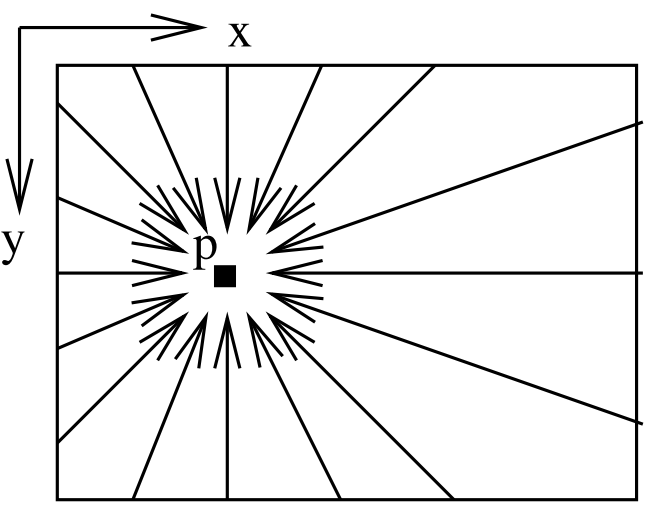
\includegraphics[scale=0.3]{sgm_paths.png}
\caption{Схема направлений оптимизации в алгоритме SGM \cite{hirschmuller2005accurate}}
\label{fig:sgm_paths}
\end{figure}

В целях предобработки пары изображений, полученных с помощью стереокамеры, нами была использована общедоступная реализация алгоритма SGM из открытой библиотеки OpenCV. В данной реализации в качестве функции схожести $C(p, D_p)$ используется сумма абсолютных разниц (SAD) в окрестности пикселя.

\subsubsection{Алгоритм AD-Census}
Данный алгоритм \cite{mei2011building} является модификацией алгоритма SGM для систем массового параллелизма, таких как графические ускорители.

В отличие от алгоритма SGM, в алгоритме AD-Census используется функция схожести, основанная на взвешенном среднем двух компонент: абсолютной разности интенсивностей (компонента AD) и расстоянии Хэмминга (компонента Census). Кроме того, авторы предлагают ряд модификаций оригинального алгоритма SGM для практического уменьшения количества требуемых вычислений.

В целях предобработки пары изображений, полученных с помощью стереокамеры, нами была использована закрытая реализация алгоритма AD-Census, выполненная инженерами компании Ланит-Терком\cite{tercom} и предоставленная нам в рамках сотрудничества компании с кафедрой системного программирования.


\subsubsection{Алгоритм CVS}
Алгоритм CVS\cite{cvs} является запатентованной разработкой компании ``Системы Компьютерного Зрения''\cite{cvs_webpage} и стал доступен нам благодаря сотрудничеству компании с кафедрой системного программирования. Данный алгоритм позволяет строить разреженную карту глубины, где значения глубины сопоставляются ключевым точкам -- пикселям на изображении, соответствующим выраженным перепадам яркости на изображении.

Ключевым преимуществом данного алгоритма является возможность реализовать его крайне эффективно, в том числе на ПЛИС\cite{cvs}.

\subsubsection{Сравнение алгоритмов построения карты глубины}

На рис. \ref{fig:compare_stereo} представлены результаты запуска рассмотренных алгоритмов расчёта карты диспаритета на одном и том же изображении. Заметно, что агоритм CVS вычисляет диспаритет лишь в небольшой доле точек. Более того, эти точки расположены неравномерно. Также заметно, что результаты работы алгоритмов SGM и AD-Census дают приблизительно одинаковый результат. Однако есть и существенные отличия. Так, в выбранной реализации алгоритма SGM нет заполнения заслонённых областей, а выбранная реализация AD-Census хуже справляется со сглаживанием плоскости дорожного полотна. Вторая проблема представляет б\'oльшую сложность для разработанного нами алгоритма детектирования препятствий, поэтому было решено для экспериментов, в которых необходимо вычисление плотной карты диспаритета, использовать реализацию SGM из библиотеки OpenCV.

\begin{figure}[htp]
\centering
\subfloat[Левое ректифицированное изображение]{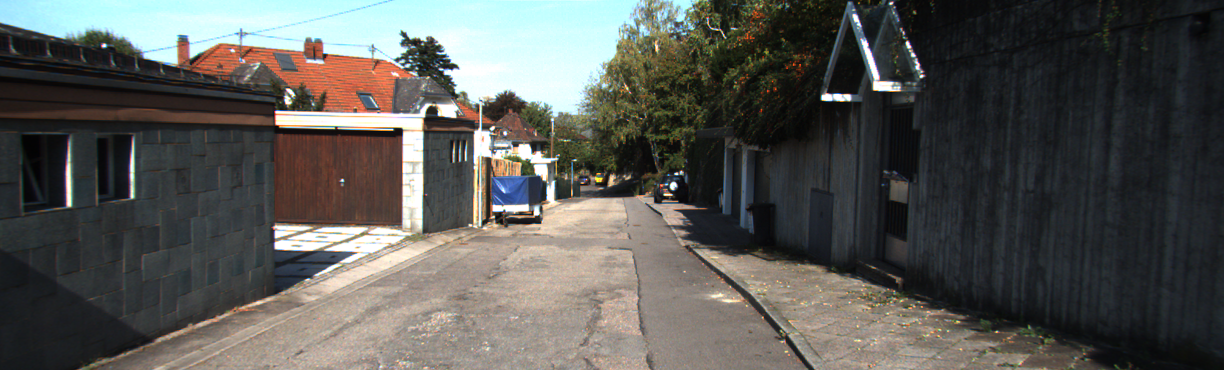
\includegraphics[scale=0.35]{ex_original.png}}\\
\subfloat[Semi-global Matching]{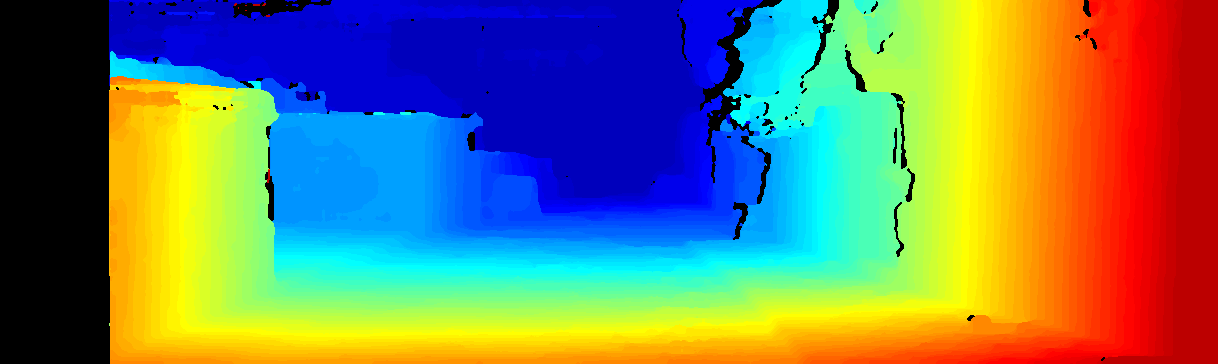
\includegraphics[scale=0.35]{ex_sgm.png}}\\
\subfloat[AD-Census]{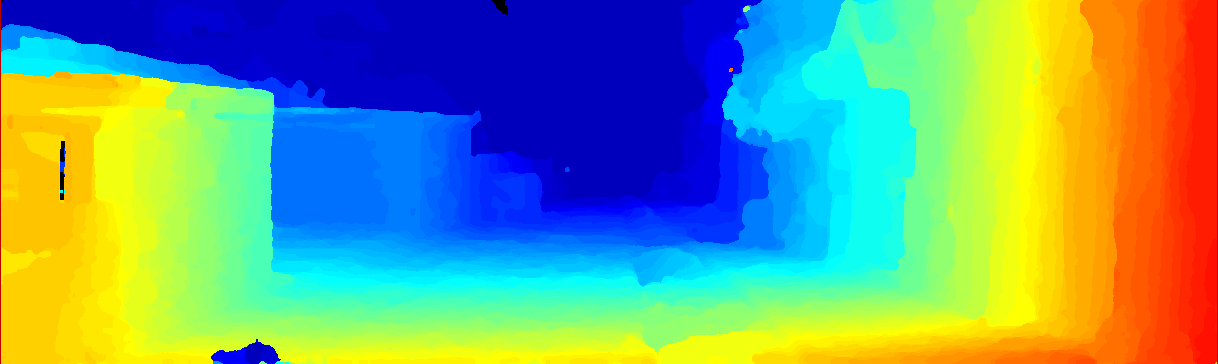
\includegraphics[scale=0.35]{ex_adcensus.png}}\\
\subfloat[CVS]{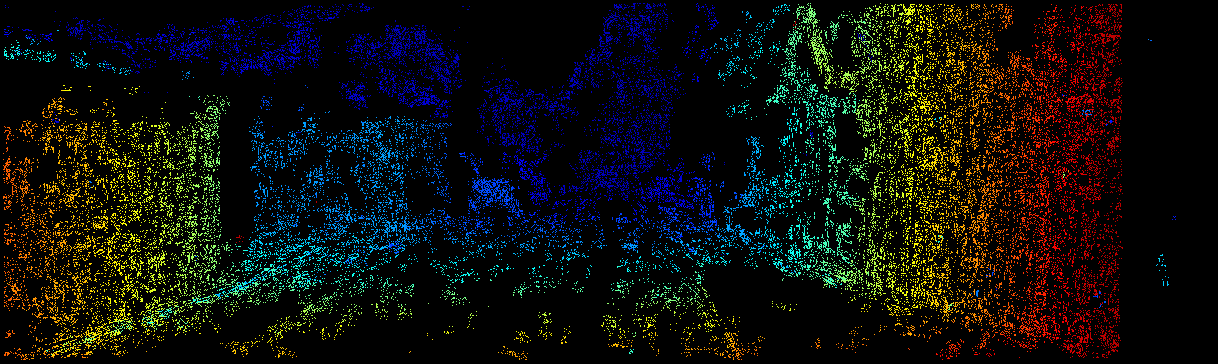
\includegraphics[scale=0.35]{ex_cvs.png}}
\caption{Результаты запуска различных алгоритмов расчёта карты диспаритета (значение диспаритета закодировано цветом)}
\label{fig:compare_stereo}
\end{figure}


\subsection{Существующие подходы к детектированию препятствий с помощью стереокамеры}

Существует большое количество исследований в области детектирования неклассифицированных объектов с помощью стереокамеры. В рамках работы было проведено исследование работ в данной области. Перечислим далее работы, наиболее релевантные нашей цели.

Авторы \cite{heinrich2002fast} предложили использовать геометрическую зависимость между оптическим потоком и расстоянием до объекта, вычисленным с помощью алгоритмов построения карты глубины. Как отмечают авторы, данный подход неустойчив к движению камер в плоскости кадра и к неточностям алгоритмов расчёта оптического потока и карты глубины. К плюсам предложенного решения можно отнести высокую скорость работы, без учёта вычисления оптического потока и расчёта карты глубины.

В работе \cite{labayrade2002real} авторы представили способ определения рельефа дорожной поверхности без использования карты глубины. Также авторы показали принципиальную возможность выделять отдельные препятствия с помощью представленного ими алгоритма. Однако точность алгоритма невысока, особенно в случае наличия большого количества препятствий на изображении. Тем не менее, способ динамического определения положения дорожного полотна, предложенный в этой работе, широко используется. В том числе, он был использован в нашем исследовании.

Развивая подход Labayrade \cite{labayrade2002real}, авторы \cite{broggi2006single} предлагают улучшения для алгоритма, позволяющие применять алгоритм в ситуациях бездорожья. Тем не менее авторы приводят только качественную оценку своего алгоритма, из которой следует вывод, что алгоритм применим только в ситуациях с небольшим количеством препятствий на изображении, как и подход Labayrade  \cite{labayrade2002real}.

В работе \cite{franke20056d} предложен подход выделения препятствий на изображении, основанный на расчёте неплотного оптического потока с помощью KLT-трекера и фильтра Калмана и расчёте неплотной карты глубины. Авторы данной работы не приводят способа выделения отдельных объектов на изображении, также в данной работе не рассмотрено выделение препятствий, не имеющих собственного движения.

В статье \cite{pfeiffer2010efficient} авторы предлагают вместо вычисления карты глубины сегментировать изображение на вертикальные полосы, для каждой из которых вычисляются две горизонтальных границы, соответствующие основанию ближайшего препятствия и его высоте. Затем, используя эту сегментацию, можно выделить объекты не прибегая к сложным вычислениям. Данный подход показался нам перспективным и многие идеи нашего исследования были заимствованы из данной работы, поэтому опишем этот алгоритм подробно.


\subsection{Динамическое определение положения плоскости дорожного полотна}\label{vdisparity_explanation}

В данной работе мы использовали оценку плоскости дорожного полотна с помощью алгоритма, предложенного в статье \cite{labayrade2002real}. Авторы предлагают для каждой строки карты диспаритетов построить гистограмму, затем получившиеся гистограммы сконкатенировать. Получившееся изображение авторы носит название ``vdisparity image''. На рис. \ref{fig:vdisp_example} приведён пример вычисления плоскости дорожного полотна. Слева направо на этом изображении представлены фрагмент исходного левого изображения, ``vdisparity image'', ``vdisparity image``, на котором пунктирной линией отмечена область, соответствующая диспаритету дороги. Поиск этой области осуществляется наложением на модель параметрической модели (в данном случае, линии), с помощью преобразования Хафа. Получившаяся линия имеет следующую интерпретацию: если точка с координатами $(x, y)$ принадлежит линии, то ожидаемое значение диспаритета плоскости дороги в строке изображения $y$ равно $x$.

\begin{figure}[htp]
\centering
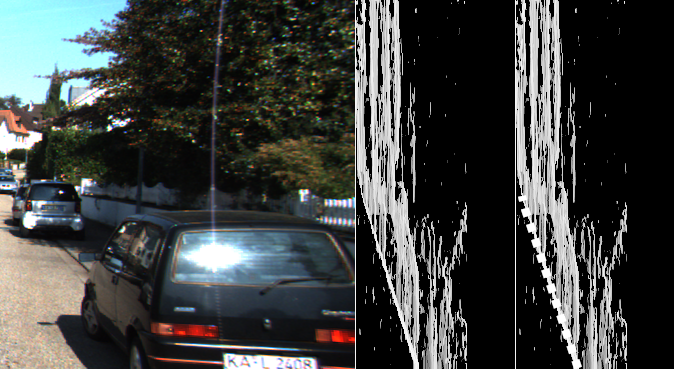
\includegraphics[width=\textwidth]{vdisp_concat.png}
\caption{Пример определения плоскости дорожного полотна}
\label{fig:vdisp_example}
\end{figure}

\subsection{Подход Stixel World} \label{sec:stixels}

Опишем данный подход \cite{pfeiffer2010efficient}, подробнее, так как он оказал существенное влияние на наше исследование.

\begin{figure}[htp]
\centering
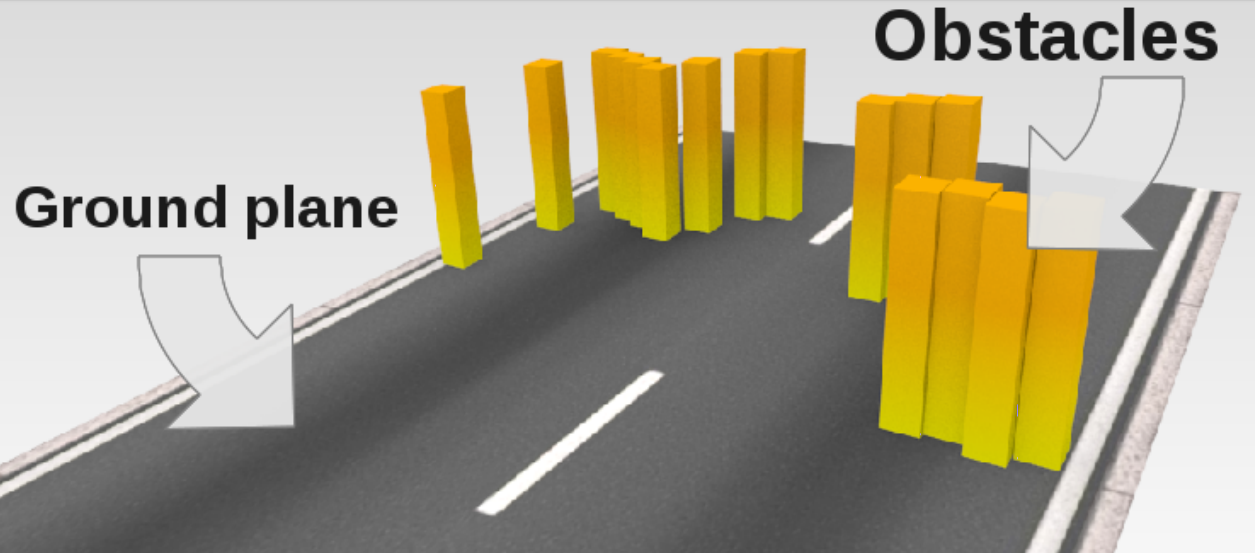
\includegraphics[width=\textwidth]{stixels_basic.png}
\caption{Упрощённое представление мира в модели Stixel World \cite{benenson2011stixels}}
\label{stixels_basic}
\end{figure}

В модели Stixel World препятствия описываются упрощённой моделью: предполагается, что любое препятствие может быть хорошо приближено параллелепипедом. В таком случае на изображении препятствия могут быть хорошо приближены набором вертикальных прямоугольников с сопоставленными им значениями глубины. На рис. \ref{stixels_basic} изображена схема упрощённой модели препятствий, принятой в модели Stixel World.

Таким образом, модель Stixel World предполагает сегментацию изображения на стиксели -- прямоугольники фиксированной ширины. Каждому стикселю соответствует 4 следующих значения.
\begin{enumerate}
\item Индекс стикселя.
\item Координата строки изображения -- нижняя граница стикселя. 
\item Координата строки изображения -- верхняя граница стикселя.
\item Значение расстояния. При этом предполагается, что расстояние одинаково до всех пикселей, принадлежащих стикселю.
\end{enumerate}

Пример сегментации изображения, получаемый с использованием модели Stixel World, представлен на рис. \ref{stixels_segm}.

\begin{figure}[htp]
\centering
\includegraphics[width=\textwidth]{/home/me/mm/master/stixels_example.png}
\caption{Пример сегментации препятствий с помощью стикселей. Цветом закодировано расстояние.}
\label{stixels_segm}
\end{figure}

Для построения модели Stixel World по двум изображениям, полученным с помощью стереокамеры, авторы предлагают минимизировать сумму двух целевых функций.

\begin{equation}\label{eq:stix_basic}
d^*_s(u) = \argmin_{d(u)}\sum_u c_s(u, d(u)) + \sum_{u_a, u_b} s_s(d(u_a), d(u_b))
\end{equation}

\begin{equation}
c_s(u, d) = c_o(u, d) + c_g(u, d)
\end{equation}

\begin{equation}\label{eq:stix_co}
c_o(u, d) = \sum_{v=v(h_o, d)}^{v(d)} c_m(u, v, d)
\end{equation}

\begin{equation}\label{eq:stix_cg}
c_g(u, d) = \sum_{v=v(d)}^{|V|} c_m(u, v, f_{ground}(v))
\end{equation}

\begin{equation}\label{eq:stix_ss}
s_s(d_a, d_b)=
\begin{cases}
  \infty, & \text{если}\ d_a < d_b - 1 \\
  c_o(u_a, d_a) & \text{если}\ d_a = d_b - 1 \\
  0, & \text{если}\ d_a > d_b - 1 \\
\end{cases}
\end{equation}

В формулах (\ref{eq:stix_basic}) -- (\ref{eq:stix_ss}) приняты следующие обозначения:

\begin{itemize}
\item $u$ -- порядковый номер стикселя,

\item $v$ -- индекс строки изображения,

\item $d^*_s$ -- вычисленное значение диспаритета для стикселя под номером $u$,

\item $h_0$ -- минимальная высота объекта на сцене, в метрах,

\item $c_m(u, v, d)$ -- значение функции схожести в точке $(u, v)$ для диспаритета $d$,

\item $f_{ground}(v)$ -- диспаритет плоскости дороги для строки $v$ изображения,

\item $u_a, u_b$ -- индексы соседних стикселей.
\end{itemize}

Также авторы предлагают способ оценки высоты объектов с помощью оценки высоты стикселей. Для этого вводится схожая целевая функция, которую мы опустим для краткости.

Такая целевая функция допускает минимизацию на ректифицированной паре изображений с помощью техник динамического программирования, что и было предложено авторами модели Stixel World.

Данный подход требует значительно больше вычислительных ресурсов, в отличие от предыдущих, однако авторы \cite{benenson2011stixels} сообщают, что алгоритм может быть оптимизирован для работы в реальном времени.

Авторами работы \cite{benenson2011stixels} была выполнена и выложена в открытый доступ реализация\cite{doppia_repo} вычисления параметров модели Stixel World для пары изображений, полученных с помощью стереокамеры. 


\subsection{Подходы к детектированию маркеров дорожной разметки}

В рамках задачи детектирования маркеров дорожной разметки было проведено большое количество исследований\cite{hillel2014recent}. Множество подходов основано на методах глубокого обучения, однако мы отказались от таких методов в силу специфики задачи.

Альтернативой являются подходы на основе классического компьютерного зрения и параметрических моделей. Простейшей параметрической моделью является прямая. Оказывается, что детектирования прямых достаточно в случае движения по автомагистралям\cite{hillel2014recent}.

Работы, связанные с параметрическими моделями, во многом схожи, поэтому здесь приведём только две наиболее релевантные. 

Подход, предложенный авторами работы \cite{song2017real} состоит из двух этапов. Сначала к изображению применяется преобразование Bird's Eye View, проецирующее плоскость камеры на плоскость дороги, затем производится выделение выраженных горизонтальных линий в пространстве Хафа, соответствующих набору маркеров дорожной разметки.

Подход, предложенный авторами работы \cite{aly2008real} во многом схож с подходом \cite{song2017real}. Однако линии задаются более сложной моделью -- в виде кубических сплайнов. Подбор параметров такой модели осуществляется с помощью алгоритма RANSAC\cite{fischler1987random}. Однако такое усложнение модели ведёт к увеличению количества шума.

\newpage
\section{Алгоритм поиска препятствий движению автомобиля}\label{sec:mystix_dense}

В данном разделе описан предложенный и реализованный в виде прототипа алгоритм поиска препятствий с помощью стереокамеры. Основные идеи данного подхода взяты из модели Stixel World \cite{pfeiffer2010efficient}, описанной в разделе \ref{sec:stixels}, однако вместо подбора параметров модели с помощью пары изображений, полученных стереокамеры, предложенный нами алгоритм производит подбор параметром модели с помощью карты диспаритета, построенное по паре изображений.

\subsection{Поиск препятствий с помощью плотной карты диспаритета}\label{sec:my_dense_stixels}

В данном разделе описан алгоритм выделения препятствий с помощью модели Stixel World, вычисленной с помощью плотной карты глубины.

Использование плотной карты глубины вместо исходной пары изображений ведёт к модификации целевой функции. В связи с тем, что расстояние до точек изображения уже вычислено, для построения модели Stixel World достаточно для каждого стикселя вычислить координаты верхней и нижней границ. Модифицированная целевая функция для оценки нижней границы стикселей имеет вид, описанный в формуле \ref{eq:mystix_basic}. Отметим, что размер левого изображения, правого изображения и карты диспаритетов мы считаем одинаковым.

В формулах (\ref{eq:mystix_basic}) -- (\ref{eq:mystix_ss}) принятны следующие обозначения, в целом соответствующие обозначениям раздела \ref{sec:stixels}.

\begin{itemize}

\item $u$ -- индекс стикселя.

\item $v$ -- индекс строки изображения.

\item $v_{bot}(u)$ -- нижняя граница стикселя с индексом $u$.

\item $v_{bot}^*(u)$ -- оптимальная нижняя граница стикселя с индексом $u$.

\item $|V|$ -- количество строк изображения.

\end{itemize}

\begin{equation}\label{eq:mystix_basic}
v_{bot}^*(u) = \argmin_{v}[\sum_u c_s(u, v) + \sum_{u_a, u_b: |u_a - u_b| = 1} s_s(v_{bot}(u_a), v_{bot}(u_b))]
\end{equation}

Формула (\ref{eq:mystix_basic}) состоит из двух слагаемых. Первое слагаемое, $c_s(u, v)$, представляет собой оценку правдоподобности наличия нижней границы препятствия в строке $v$ стикселя $u$ и имеет вид, описанный в формулах (\ref{eq:mystix_cost_bottom}) -- (\ref{eq:mystix_cg}). 

\begin{equation}\label{eq:mystix_cost_bottom}
c_s(u, v) = c_o(u, v) + c_g(u, v)
\end{equation}

\begin{equation}\label{eq:mystix_co}
c_o(u, v) = \sum_{v'=v(h_o, d(u, v))}^{v} |d(u, v) - d(u, v')|
\end{equation}

\begin{equation}\label{eq:mystix_cg}
c_g(u, v) = \sum_{v'=v}^{|V|} |d(u, v) - d_{ground}(u, v')|
\end{equation}

В формулах (\ref{eq:mystix_cost_bottom}) -- (\ref{eq:mystix_cg}) приняты следующие обозначения.

\begin{itemize}

\item $c_o(u, v)$ -- функция правдоподобности наличия препятствия в стикселе $u$ на строке изображения $v$.

\item $c_g(u, v)$ -- функция правдоподобности отсутствия препятствия в стикселе $u$ в во всех строках изображения $v' : v' > v$.

\item $d_{ground}(u, v)$ -- ожидаемое значение диспаритета в стикселе $u$, в строке $u$ для плоскости дорожного полотна.

\item $d(u, v)$ -- медиана значений в строке $v$ карты диспаритетов, соответствующих стикселю $u$, т.е. медиана значений карты диспаритетов на позициях $(w * u, v)\dots (w * (u + 1) - 1, v)$, где $w$ -- предопределённая ширина стикселя.

\end{itemize}

Второе слагаемое формулы (\ref{eq:mystix_basic}) представлено в формуле (\ref{eq:mystix_ss}). $c_{jump}$ в этой формуле обозначает наперёд заданный порог.

\begin{equation}\label{eq:mystix_ss}
s_s(v_a, v_b)=
\begin{cases}
  \infty,     & \text{если}\ |v_a - v_b| > c_{jump} \\
  |v_a - v_b| & \text{иначе}
\end{cases}
\end{equation}

Функция оценки верхней границы стикселей имеет схожий вид и представлена в формулах (\ref{eq:mystix_height_basic}) -- (\ref{eq:mystix_cost_h}).

\begin{equation}\label{eq:mystix_height_basic}
v_{top}^*(u) = \argmin_{v}\sum_u c_s^h(u, v) + \sum_{v_{top}^a, v_{top}^b} s_s(v_{top}^a, v_{top}^b)
\end{equation}

\begin{equation}\label{eq:mystix_cost_h}
c_s^h(u, v) = \sum_{v'=v}^{v_{bot}} |d(u, v) - d(u, v')| - k * |d(u, v_{bot})| * |v' - v|
\end{equation}

Для вычисления функции (\ref{eq:mystix_cg}) требуется знание диспаритета плоскости дорожного полотна в стикселе $u$ в строке $v$. Для этого мы используем подход, предложенный в статье \cite{labayrade2002real} и описанный в разделе \ref{vdisparity_explanation}.

В листинге \ref{alg:stixels} представлен псевдокод алгоритма сегментации карты диспаритетов согласно модели Stixel World.

На рис. \ref{fig:stix_small} и \ref{fig:stix_offroad} приведены примеры работы алгоритма в двух ситуациях. На рис. \ref{fig:stix_small} алгоритм применён для детектирования небольшого объекта (детской игрушки), на рис. \ref{fig:stix_offroad} верхняя граница стикселей не показана, вместо этого выделена область, ограниченная нижней границей изображения и нижней границей стикселей.



\begin{algorithm}[H]
\caption{Сегментация плотной карты диспаритета согласно модели Stixel World}
\label{alg:stixels}
\begin{algorithmic}[1]
\Require Карта диспаритета, ширина стикселя
\Ensure Множество стикселей, описывающих карту глубины согласно модели Stixel World
\State Вычислить значение $d_{ground}(u, v)$, используя алгоритм из раздела \ref{vdisparity_explanation}.
\ForAll{$(u, v)$}
\State Вычислить значение $c_s(u, v)$, заданное функцией (\ref{eq:mystix_cost_bottom}).
\EndFor
\State С помощью динамического программирования вычислить значения $v_{bot}^*(u_1) \dots v_{bot}^*(u_n)$, заданные функцией (\ref{eq:mystix_basic}).
\ForAll{$(u, v)$}
\State Вычислить значение $c_s^h(u, v)$, заданное функцией (\ref{eq:mystix_cost_h}).
\EndFor
\State С помощью динамического программирования вычислить значения $v_{top}^*(u_1) \dots v_{top}^*(u_n)$, заданные функцией (\ref{eq:mystix_height_basic}).
\end{algorithmic}
\end{algorithm}

\begin{figure}[H]
\centering
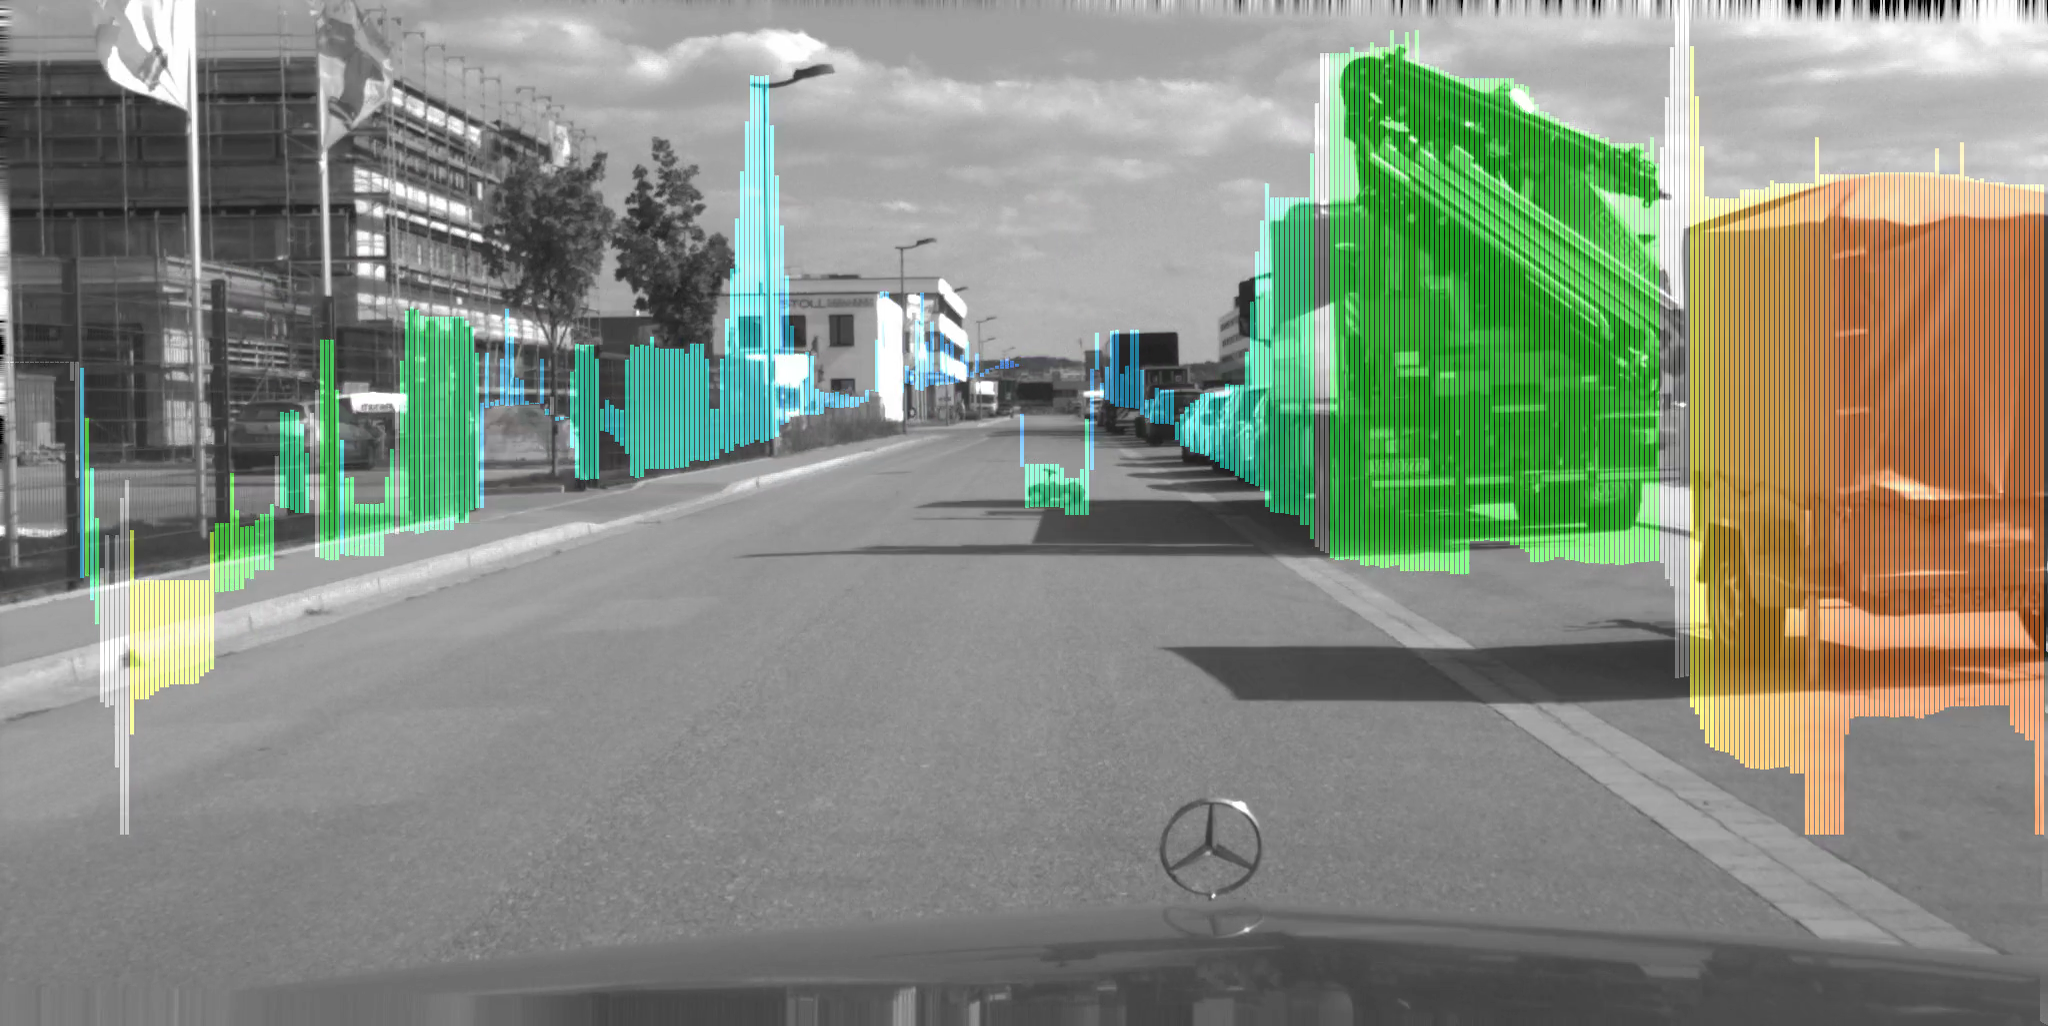
\includegraphics[width=\textwidth]{small_object.png}
\caption{Сегментация изображения согласно модели Stixel World. Цветом закодировано расстояние.}
\label{fig:stix_small}
\end{figure}

\begin{figure}[H]
\centering
\includegraphics[width=\textwidth]{offroad.png}
\caption{Выделение области, безопасной для движения, с помощью сегментации согласно модели Stixel World.}
\label{fig:stix_offroad}
\end{figure}

\newpage

\subsection{Поиск препятствий с помощью разреженной карты диспаритета}\label{sec:my_sparse_stixels}

Реализация алгоритма подбора параметров модели Stixel World для разреженной карты диспаритета представляет интерес, в связи с наличием высокоэффективных алгоритмов вычисления разреженной карты диспаритета, например, CVS\cite{cvs}. Благодаря сотрудничеству с компанией ``Системы компьютерного зрения'' нам стала доступна реализация алгоритма CVS, которая и была использована в наших экспериментах.

Прямой перенос алгоритма из раздела \ref{sec:my_dense_stixels} на карту глубины, вычисленную с помощью алгоритма CVS затруднителен, так как дорожное полотно зачастую низкотекстурировано. Это приводит к тому, что количество точек дорожного полотна на изображении, в которых вычислено значение диспаритета, оказывается небольшим по сравнению с количеством точек, принадлежащим препятствиям. Следствием этого является зачастую неверно вычисленные параметры модели плоскости земной поверхности.

В связи с этим мы модифицировали исходный алгоритм. 

Идея модифицированного алгоритма состоит в следующем. Оценка плоскости дорожного полотна с помощью vdisparity заменяется оценкой с помощью алгоритма RANSAC. При этом для подбора параметров модели плоскости дорожного полотна используются только те точки изображения, в которых вычислено значение диспаритета и которые находятся на небольшом удалении в смысле нормы $l_1$ от середины нижнего края изображения. Связано это с тем, что в случае расположения камеры на лобовом стекле автомобиля и предварительном удалении капота автомобиля с изображения, как это сделано во всех использованных нами наборах данных, середина нижнего края изображения соответствует точке непосредственно перед автомобилем. То есть, в случае, если соблюдена нужная дистанция, эти точки соответствуют только дороге.

Далее происходит вычисление нижней границы стикселей в манере алгоритма из раздела \ref{sec:my_dense_stixels}, однако в связи с низкой плотностью карты диспаритета целевой функционал претерпел следующие изменения. С использованием модели плоскости дорожного полотна, вычисленной ранее, точки изображения, для которых было вычислено значение диспаритета помечаются как ``дорога'', если они удовлетворяют модели плоскости дорожного полотна и ``препятствие'' иначе. Далее целевая функция нижней границы вычисляется аналогично формуле (\ref{eq:mystix_basic}), однако первое слагаемое этой формулы заменяется на формулу (\ref{eq:mysparsestix_cost_bottom}). В формуле (\ref{eq:mysparsestix_cost_bottom}) $object(u, v')$ обозначает количество точек изображения в строке $v'$ стикселя $u$, помеченных как ``препятствие'', аналогично $ground(u, v')$ обозначает количество точек изображения в строке $v'$ стикселя $u$, помеченных как ``дорога''. Отметим, что такая функция может быть эффективно вычислена с использованием нарастающих сумм.

\begin{equation}\label{eq:mysparsestix_cost_bottom}
c_s(u, v) = \sum_{v'}^{|V|} object(u, v') + \sum_{0}^{v'} ground(u, v')
\end{equation}

Вычисление верхней границы стикселей для разреженной карты глубины нами не проводилось, так как, с одной стороны, оно не является необходимым для детектирования объектов, с другой стороны, является недостаточно робастным в следствие разреженности стерео.

Псевдокод модифицированного алгоритма приведён в листинге \ref{alg:sparse_stixels}.

\begin{algorithm}[H]
\caption{Сегментация разреженной карты диспаритета согласно модели Stixel World}
\label{alg:sparse_stixels}
\begin{algorithmic}[1]
\Require Разреженная карта диспаритета, ширина стикселя
\Ensure Множество нижних границ стикселей, описывающих карту глубины согласно модели Stixel World
\State Из всех точек карты диспаритета выбрать те, для которых выполнено неравенство $max(|y_i - height_{img}|, |x_i - (width_{img} / 2) |) < C$. Обозначим множество таких точек $P_{road}$.
\State Вычислить нормаль к плоскости дороги, максимизируя количество точек из множества $P_{road}$, принадлежащих плоскости дороги при помощи алгоритма RANSAC.
\State Вычислить карту стоимости согласно формуле (\ref{eq:mysparsestix_cost_bottom}).
\State С помощью динамического программирования вычислить значения $v_{bot}^*(u_1) \dots v_{bot}^*(u_n)$, заданные функцией (\ref{eq:mystix_basic}).
\end{algorithmic}
\end{algorithm}

На рис. \ref{fig:sparse_stixels_steps} представлена визуализация шагов алгоритма, описанного в данном разделе. На рис. \ref{fig:sparse_stixels_steps}.b видно, что количество точек на дороге невелико. Как упоминалось выше, это может привести к неверному определению плоскости дороги. Для того, чтобы снизить этот эффект, возможно считать положение плоскости дорого относительно камеры постоянным, что, однако, приводит к существенному снижению точности определения нижней границы объекта в типичном случае.

\begin{figure}[htp]
\centering
\subfloat[Левое ректифицированное изображение]{\includegraphics[scale=0.35]{left.png}}\\
\subfloat[Карта диспаритета, вычисленная с помощью алгоритма CVS]{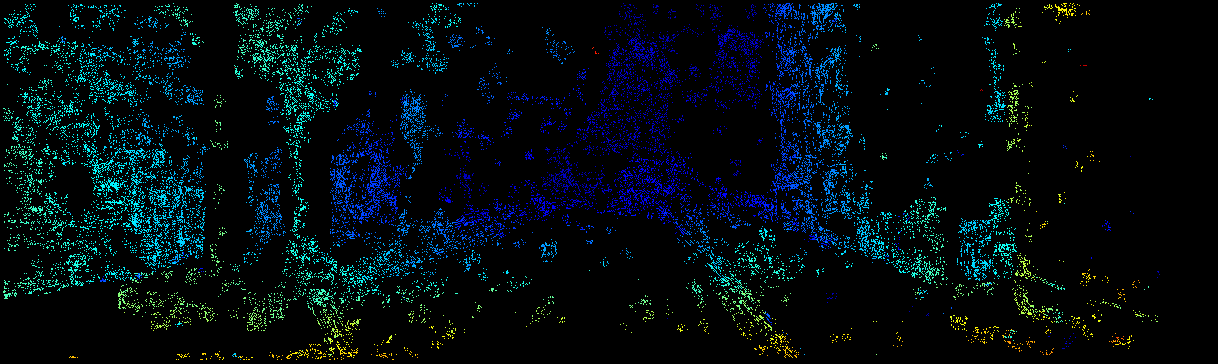
\includegraphics[scale=0.35]{sparse_stixels_stereo.png}}\\
\subfloat[Результат разделения неплотного облака стерео-точек на классы ``дорога'' и ``препятствия'']{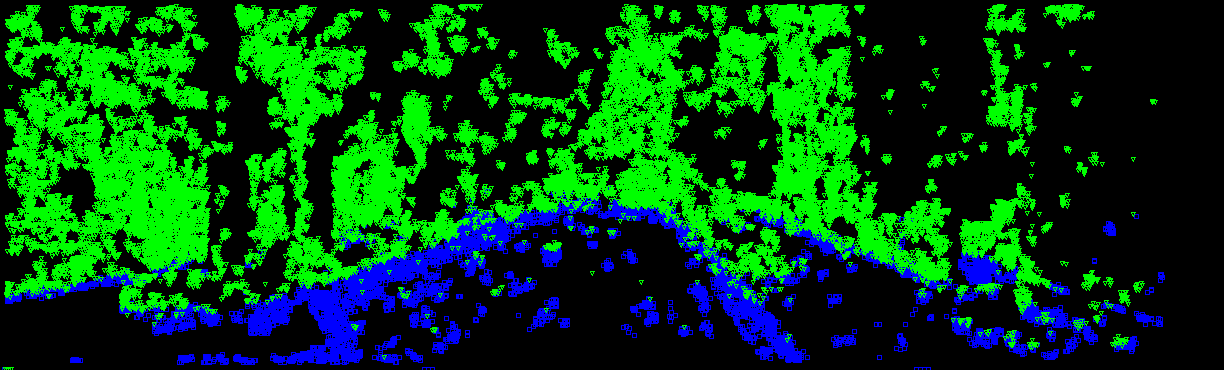
\includegraphics[scale=0.35]{plane.png}}\\
\subfloat[Результат оценки нижней границы стикселей]{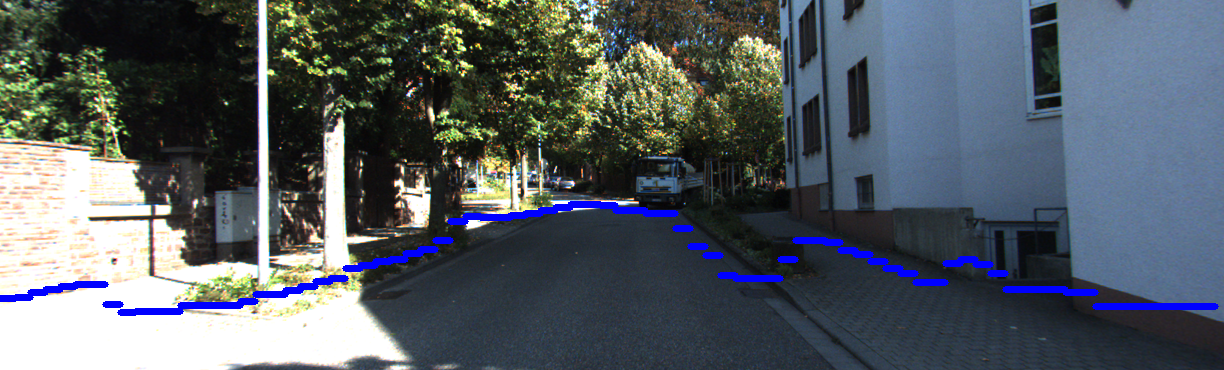
\includegraphics[scale=0.35]{left_stix.png}}
\caption{Этапы вычисления нижней границы стикселей с помощью алгоритма из листинга \ref{alg:sparse_stixels}}
\label{fig:sparse_stixels_steps}
\end{figure}

\newpage
\section{Алгоритм детектирования маркеров дорожной разметки}

На основе алгоритме из статьи \cite{aly2008real} нами был разработан алгоритм детектирования маркеров дорожной разметки. Данный алгоритм рассчитан на поиск маркеров дорожной разметки в виде прямых линий. Алгоритм включает в себя защиту от ложных срабатываний на некоторых дополнительных элементах разметки: пешеходный переход, остановка общественного транспорта, маркеры направлений движения. Кроме того, с помощью разработанного алгоритма возможно детектировать, например, бордюр, что необходимо в условиях движения в условиях города.

Псевдокод разработанного алгоритма представлен в листинге \ref{alg:markers}.

\begin{algorithm}
\caption{Выделение маркеров дорожной разметки на изображении}\label{alg:euclid}
\label{alg:markers}
\begin{algorithmic}[1]
\Require цветное изображение $img$, калибровочные данные для камеры
\Ensure Маска для изображения $img$, на которой отличные от нуля значения соответствуют маркерам дорожной разметки
\State Применить к $img$ преобразование Bird's Eye View.
\State Преобразовать изображение в пространство HSV и извлечь канал Value, обозначим это новое изображение $imgHsvValue$.
\State Применить морфологическое размыкание к изображению $imgHsvValue$ для удаления недостаточно тонких линий.
\State Вычислить в каждой точке $imgHsvValue$ значение оператора Собеля, обозначим получившееся изображение $imgSobel$.
\State На $imgSobel$ приравнять к нулю все точки, направление градиента в которых существенно отличается от горизонтального.
\State Разбить $imgSobel$ на непересекающиеся прямоугольники одинакового размера, обозначим каждый такой прямоугольник $Rect(i, j)$.
\ForAll{$(i, j)$}
\State Пометим $Rect(i, j)$ как содержащий разметку, если сумма пикселей, попавших в этот прямоугольник больше порога.
\EndFor
\State Интерпретируя центры $Rect(i, j)$ как точки на изображении, с помощью алгоритма RANSAC поочерёдно извлекаем все линии разметки.
\end{algorithmic}
\end{algorithm}

Отметим, что отсутствие срабатываний на пешеходных переходах и на маркерах направлений движения достигается за счёт строки 3 листинга, а отсутствие срабатываний на остановках общественного транспорта достигается за счёт строки 5.

На рис. \ref{fig:lanes_pipline} изображены промежуточные результаты алгоритма. Слева направо на изображении представлены результаты после шагов 5, 9, 10. 

\begin{figure}[H]
     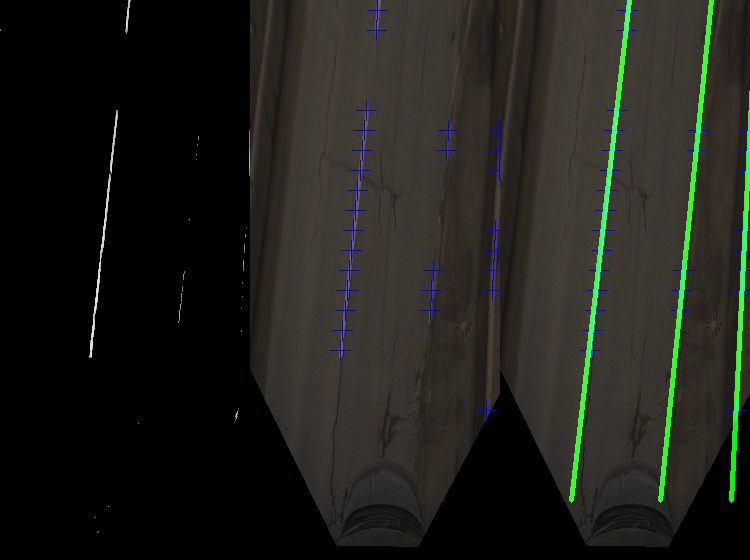
\includegraphics[width=\textwidth]{lanes_pipeline.png}
     \caption{Пример работы алгоритма выделения маркеров дорожной разметки}
     \label{fig:lanes_pipline}
\end{figure}


\newpage
\section{Апробация}

\subsection{Данные}

Для оценки качества разработанных алгоритмов были выбраны следующие наборы данных.
\begin{itemize}
\item Тестовый набор для алгоритмов детектирования объектов KITTI \cite{Geiger2012CVPR}.
\item Тестовый набор для алгоритмов детектирования маркеров дорожной разметки TuSimple \cite{tusimple}.
\item Тестовый набор для алгоритмов детектирования маркеров дорожной разметки ``Петергоф'', собранный специалистами компании Ланит-Терком и предоставленный нам для оценки алгоритма.
\end{itemize}

Набор данных KITTI состоит из приблизительно 7000 изображений, полученных с помощью стереокамеры, установленной на крыше автомобиля. Изображения были получены в рамках движения автомобиля по дорогам общего пользования Германии как в городской среде, так и в сельской местности, в различных погодных условиях. Каждое изображение проаннотировано прямоугольниками, описанными вокруг объектов, принадлежащих следующим классам: велосипедист, пешеход и автомобиль.

Пример изображения из набора данных KITTI представлен на рис. \ref{fig:ex_kitti}.

\begin{figure}[htp]
\centering
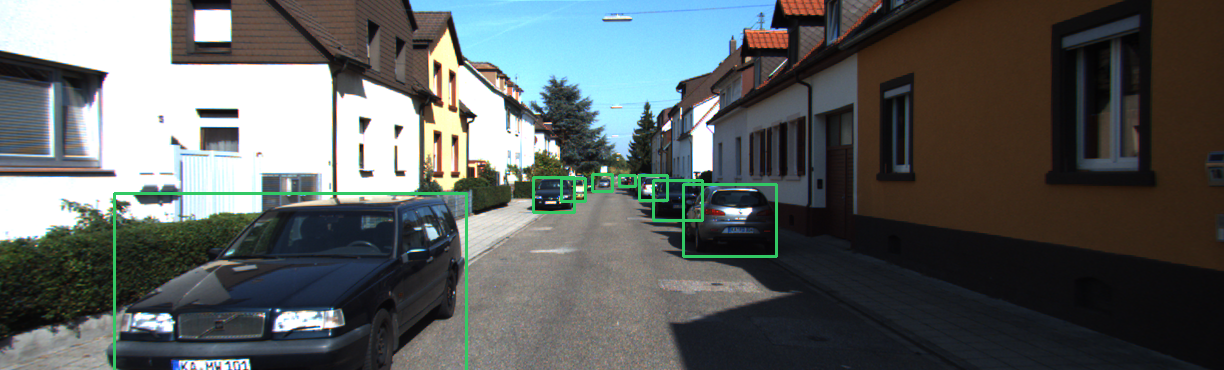
\includegraphics[width=\textwidth]{kitti_ex.png}
\caption{Пример аннотированного изображения из набора данных KITTI}
\label{fig:ex_kitti}
\end{figure}

Набор данных TuSimple представляет собой набор из 358 изображений, снятых камерой, закреплённой на автомобиле в рамках проезда автомобиля по дорогам общего пользования. Для каждого изображения присутствует аннотация, содержащая маркеры дорожной разметки. В аннотации присутствует не более пяти маркеров: два маркеров для текущей полосы движения автомобиля, два для соседних полос и пятый маркер для случая перестроения из одной полосы в другую, когда невозможно определить, какая полоса является текущей.

Пример изображения из набора TuSimple  представлен на рис. \ref{fig:ex_tusimple}.

\begin{figure}[htp]
\centering
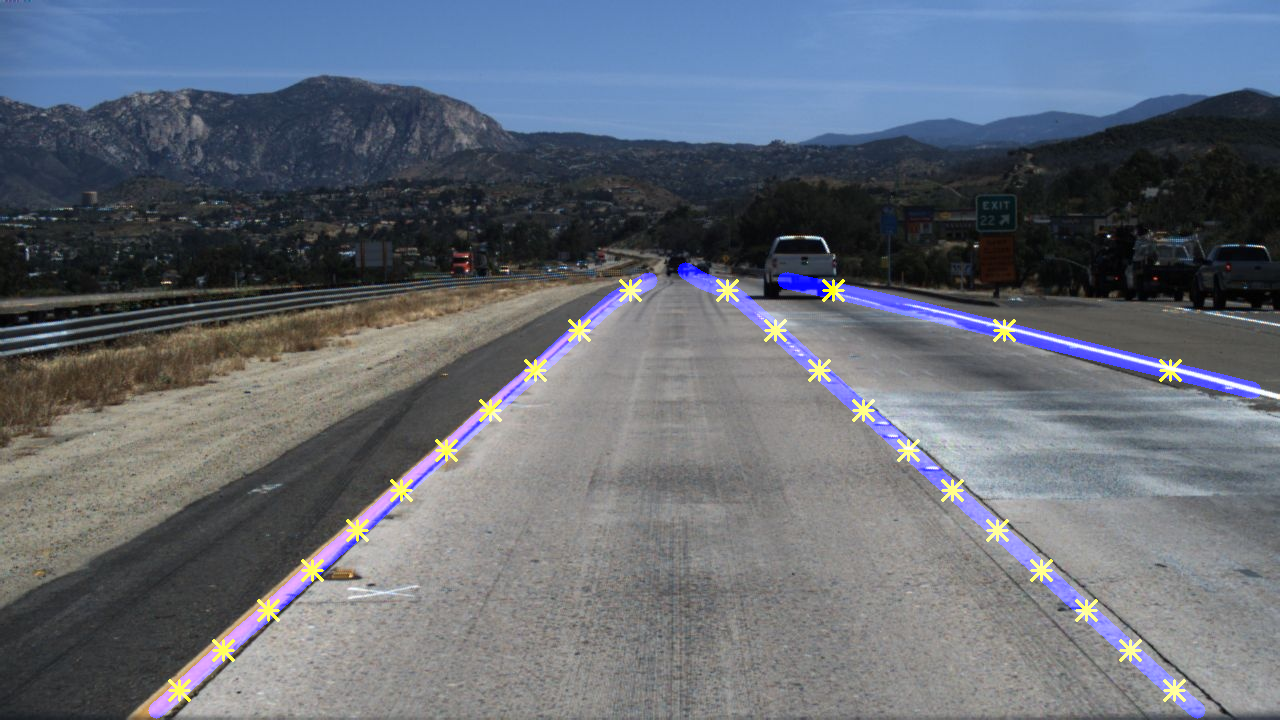
\includegraphics[width=\textwidth]{ex_tusimple.png}
\caption{Пример аннотированного изображения из набора данных TuSimple}
\label{fig:ex_tusimple}
\end{figure}

Набор данных Петергоф, представляет собой видеопоследовательность длительностью 5 минут из 5000 кадров, записанную в рамках движения автомобиля по дороге г. Петергофа. Отличительной особенностью этой последовательности является наличие бордюров, заменяющих крайние маркеры дорожной разметки. Каждый 50-й кадр этой последовательности был нами размечен: на изображении были выделены в виде маски маркеры дорожной разметки, аналогично последовательности TuSimple. При этом бордюры мы также считали маркерами разметки.

Пример изображения из набора Петергоф  представлен на рис. \ref{fig:ex_mm}.

\begin{figure}[htp]
\centering
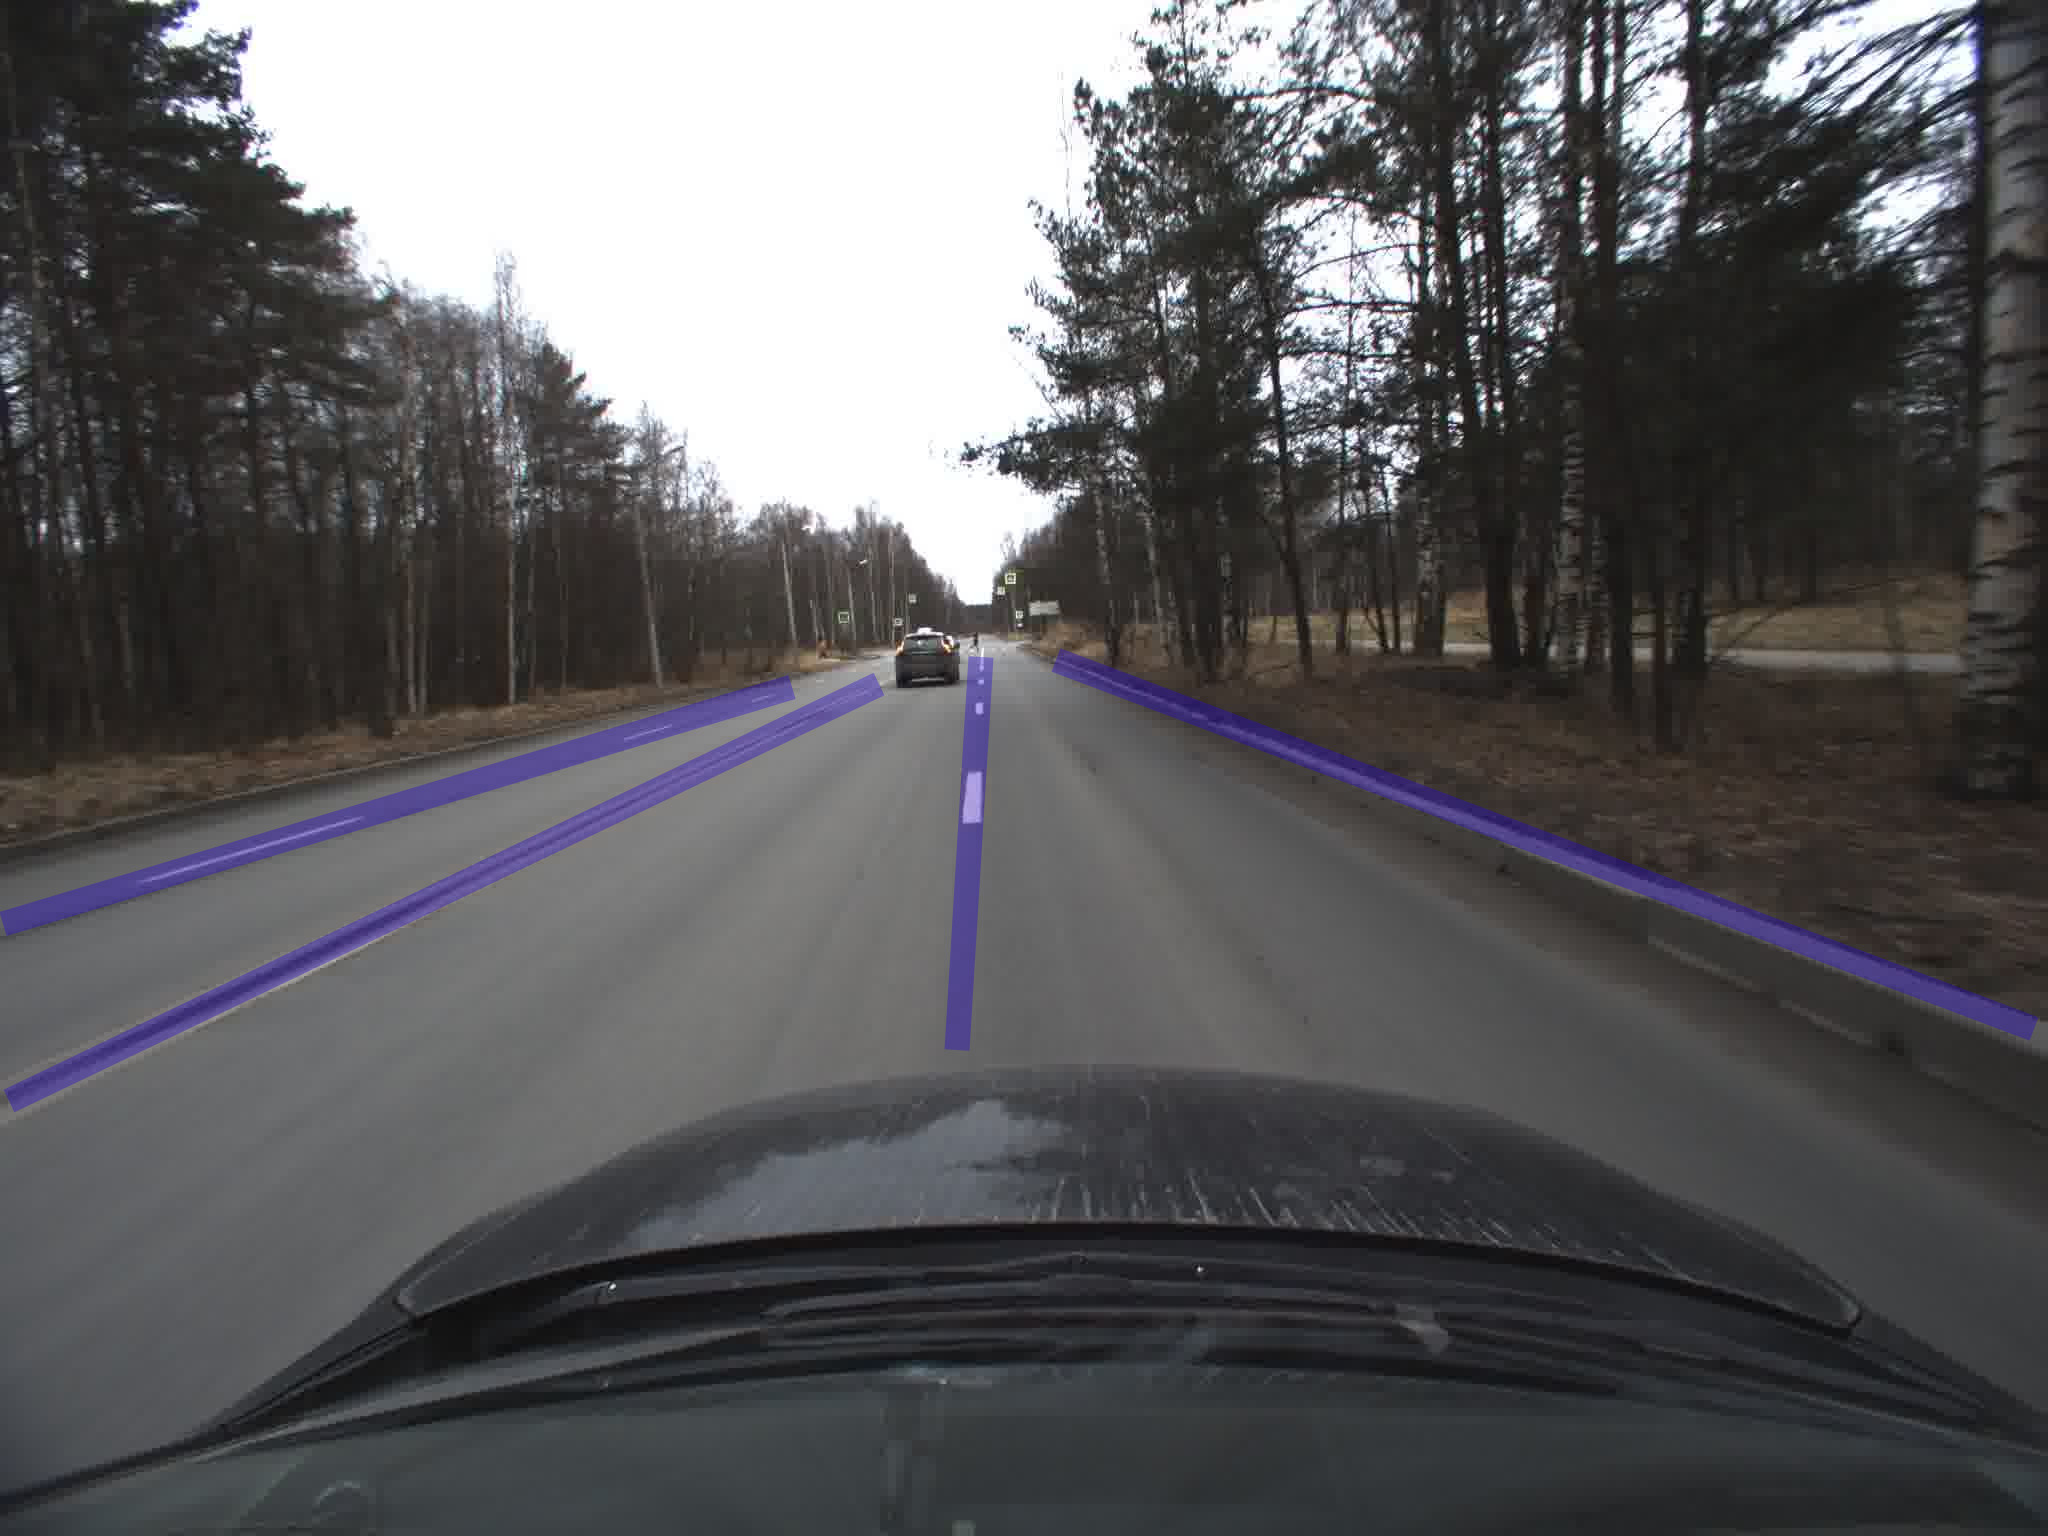
\includegraphics[scale=0.2]{ex_mm.jpg}
\caption{Пример аннотированного изображения из набора данных Петергоф}
\label{fig:ex_mm}
\end{figure}

\subsection{Оценка качества работы алгоритмов}

\subsubsection{Методика оценки алгоритма детектирования препятствий}

Так как выбранные наборы данных содержат аннотацию в виде описывающих прямоугольников, было решено применить следующий способ оценки алгоритма. 
\begin{itemize}
\item Подобрать параметры модели Stixel World для изображения, т.е. вычислить набор стикселей.
\item Для каждого описанного прямоугольника из всех стикселей выбрать те, горизонтальная координата которых заключена между левой и правой границей прямоугольника.
\item Для выбранных стикселей вычислить медиану нижней границы. Обозначим эту медиану $v_{predicted}$. Обозначим координату нижней границы прямоугольника $v_{expected}$.
\item Далее, в зависимости от значения $v_{diff} = v_{predicted} - v_{expected}$, мы рассматриваем три случая:
\begin{enumerate}
\item $|v_{diff}|   < 0.2 * bb_{height}$    -- препятствие обнаружено,
\item $\ v_{diff}\  < 0.2 * bb_{height}$  -- препятствие не обнаружено,
\item $\ v_{diff}\  > 0.2 * bb_{height}$  -- обнаружено препятствие ниже.
\end{enumerate}
\end{itemize}

В наборе данных KITTI присутствует большое количество вырожденных случаев, когда в следствие перекрытий объекту соответствует слишком малое количество пикселей. Такие объекты, как правило, расположены на горизонте и не имеют достаточного параллакса для их выделения с помощью алгоритмов стереозрения. Кроме того, расчёт карты диспаритета затруднителен на краях изображения. В связи с этим было решено исключить из тестовой выборки следующие объекты.
\begin{itemize}
\item Объекты, ширина или высота описывающего прямоугольника для которых не превышает 25 пикселей.
\item Объекты, центр которых расположен на расстоянии менее 200 пикселей от вертикального края изображения.
\end{itemize}

\subsubsection{Методика оценки алгоритма детектирования маркеров дорожной разметки}

На наборе данных TuSimple нами принята следующая методика оценки результата.

\begin{itemize}
\item С помощью разработанного нами алгоритма вычислить и сохранить предполагаемые положения маркеров дорожной разметки.
\item Для каждого найденного нашим алгоритмом маркера выполнить поиск в аннотации размеченного положения маркера, с которым есть пересечение на 50 и более процентов.
\item Если такой маркер из аннотации был найден, пометить его как обнаруженный.
\item Если такой маркер из аннотации не был найден, считать найденный нашим алгоритмом маркер ложным срабатыванием.
\item Если для какого-то маркера из аннотации не нашлось обнаруженного нашим алгоритмом маркера, считать, что маркер из аннотации не был обнаружен.
\end{itemize}

Кроме того, два ближайших к центру изображения относительно горизонтальной оси маркера из аннотации мы считаем границами собственной полосы, что позволяет разделить маркеры на два класса: маркеры собственной полосы и маркеры соседних полос.

\subsubsection{Результаты оценки алгоритма детектирования препятствий}

В таблице \ref{tab:no_filter_occ} представлены результаты сравнения нашей реализации подбора параметров модели Stixel World с реализацией\cite{doppia_repo}. Столбец ``Dense'' соответствует результату алгоритма из раздела \ref{sec:my_dense_stixels}, столбцы ``SparseR'' и ``SparseC'' соответствуют результату алгоритма из раздела \ref{sec:my_sparse_stixels}, при этом в ``SparseR'' использован подбор параметров плоскости дорожного полотна с помощью алгоритма RANSAC, а в ``SparseC'' плоскость дороги принята постоянной для всех изображений. Столбец Benenson et al. соответствует открытой реализации \cite{doppia_repo}. Строка ``перекрытие'' соответствует случаю ``обнаружен объект ниже''. Это означает, что для этих объектов стиксели, соответствующие столбцам прямоугольника, описанного вокруг объекта, имеют нижнюю границу существенно ниже, чем нижняя граница описывающего прямоугольника. 

Видно, что как в нашей реализации, так и в реализации Benenson et al. большое количество объектов находится в строке ``перекрытие''. Связано это может быть с двумя причинами: либо на изображении действительно находится препятствие, расположенное ниже объекта, заданного описанным прямоугольником, либо имеется ложное срабатывание. Отделить один случай от другого возможно только для объектов, перекрытых объектами, присутствующими в разметке. Для этого необходимо удалить из тестового множества все такие прямогуольники $a_i$, что существует $b_i$, отличный от него, пересекающийся с ним и имеющий нижнюю границу ниже, чем нижняя граница $a_i$. Результаты работы алгоритмов на таком усечённом наборе данных приведены в таблице \ref{tab:filter_occ}. Обозначения повторяют обозначения таблицы \ref{tab:no_filter_occ}.

Заметно, что и на исходном наборе данных, и на усечённом, наша реализация выигрывает в количестве обнаруженных объектов. Тем не менее, результаты запуска на наборе данных KITTI показали, что большинство неверных результатов нашего алгоритма обусловлено двумя причинами.
\begin{itemize}
\item Наличие артефактов на карте диспаритета, представляющих собой области на карте диспаритета, имеющие неверное, либо вовсе не имеющие значения диспаритета. Артефакты возникают, как правило, на зеркальных поверхностях и в засвеченных областях изображения и связаны с нарушением условий, необходимых для корректной работы алгоритмов расчёта карты диспаритета. 
\item Неверная оценка плоскости дороги. Выбранная нами модель плоскости дороги слишком проста и не в состоянии корректно описать дорожное полотно в некоторых ситуациях. Например, при наличии крена. Кроме того, в виду наличия большого количества объектов на сцене, подбор параметров модели дорожного полотна с использованием подхода vdisparity может привести к недостаточно точным значениям параметров. Также для случая неплотного стерео к неверной оценке плоскости дорожного полотна может привести недостаточная текстурированность дороги, необходимая для качественной работы алгоритма CVS.
\end{itemize}

\begin{table}
\center
\begin{tabular}{|c|c|c|c|c|}
\hline
	 & Dense & SparseR & SparseC & Benenson et al. \\
\hline
	Обнаружено 			& 15780 & 11889 & 12635 & 10168\\
\hline
	Не обнаружено 		& 355   & 4116  & 3714 & 9315\\
\hline
	Перекрытие			& 5692  & 5822  & 5478 & 2344\\
\hline
\end{tabular}
\caption{Сравнение реализаций модели Stixel World без фильтрации перекрытий}
\label{tab:no_filter_occ}
\end{table}

\begin{table}
\center
\begin{tabular}{|c|c|c|c|c|}
\hline
						 & Dense & SparseR & SparseC & Benenson et al. \\
\hline
	Обнаружено 			& 11167 & 7738 & 7817 & 6164\\
\hline
	Не обнаружено 		& 271   & 2891 & 2983 & 6505\\
\hline
	Перекрытие			& 1868  & 2677 & 2506 & 637\\
\hline
\end{tabular}
\caption{Сравнение реализаций модели Stixel World с фильтрацией перекрытий}
\label{tab:filter_occ}
\end{table}

\subsubsection{Результаты оценки алгоритма детектирования маркеров дорожной разметки}

В таблице \ref{tab:lanes_tusimple} представлены результаты запуска разработанного нами алгоритма детектирования маркеров дорожной разметки на наборе данных TuSimple. Из этой таблицы, например, видно, что точность детектирования маркеров собственной полосы выше, что неудивительно, так как этим маркерам соответствует большее число пикселей изображения.

В таблице \ref{tab:lanes_peterhof} представлены результаты запуска алгоритма на последовательности Петергоф. Видно, что процент верно обнаруженных маркеров собственной полосы (включая бордюры), так же высок, как и на последовательности TuSimple. Кроме того, уровень ложных срабатываний достаточно низок. Однако, снизился также и процент обнаруженных маркеров соседних полос движения.

\begin{table}[H]
\center
\begin{tabular}{|c|c|c|}
\hline
			& Собственная полоса & Несобственная полоса \\
\hline
	Обнаружено				& 634 & 196\\
\hline
	Не обнаружено			& 80  & 208\\
\hline
	Ложное срабатывание		& \multicolumn{2}{c|}{98}\\
\hline
\end{tabular}
\caption{Результаты работы алгоритма детектирования маркеров дорожной разметки на наборе данных TuSimple}
\label{tab:lanes_tusimple}
\end{table}

\begin{table}
\center
\begin{tabular}{|c|c|c|}
\hline
			& Собственная полоса & Несобственная полоса \\
\hline
	Обнаружено				& 146 & 16\\
\hline
	Не обнаружено			& 42  & 63\\
\hline
	Ложное срабатывание		& \multicolumn{2}{c|}{4}\\
\hline
\end{tabular}
\caption{Результаты работы алгоритма детектирования маркеров дорожной разметки на наборе данных Петергоф}
\label{tab:lanes_peterhof}
\end{table}

Улучшение качества детектирования на последовательности Петергоф связано с тем, что на этой последовательности маркеры дорожной рзметки чётко видны, в то время как на последовательности TuSimple качетсво маркеров варьируется. Это позволяет сделать вывод, что в условиях наличия качественной дорожной разметки, разработанный алгоритм справляется с возложенной на него задачей. 

На рис. \ref{fig:lane_det_fails} приведены некоторые случаи ошибок разработанного алгоритма. Так, заметно, что в случае недостаточно качественной разметки данный алгоритм не справляется с детектированием полосы. Кроме того, такие элементы как край дороги, либо полосы на объектах определённой ширины могут быть восприняты в качестве маркеров дорожной разметки. С первой проблемой справиться возможно только путём существенных модификаций алгоритма. Например, добавлением новых случаев. Вторая проблема теоретически может быть решена, например, путём интеграции с алгоритмами из раздела \ref{sec:mystix_dense}. А именно в качестве предобработки возможно удалить с изображения область, соответствующую препятствиям и выполнять поиск маркеров в оставшейся области. Нами проводились соответствующие эксперименты, которые показали улучшение качества детектирования маркеров дорожной разметки, однако в нашем распоряжении не оказалось убедительного набора данных, чтобы достоверно подтвердить эффективность такого подхода.

\begin{figure}[htp]
\centering
\subfloat[]{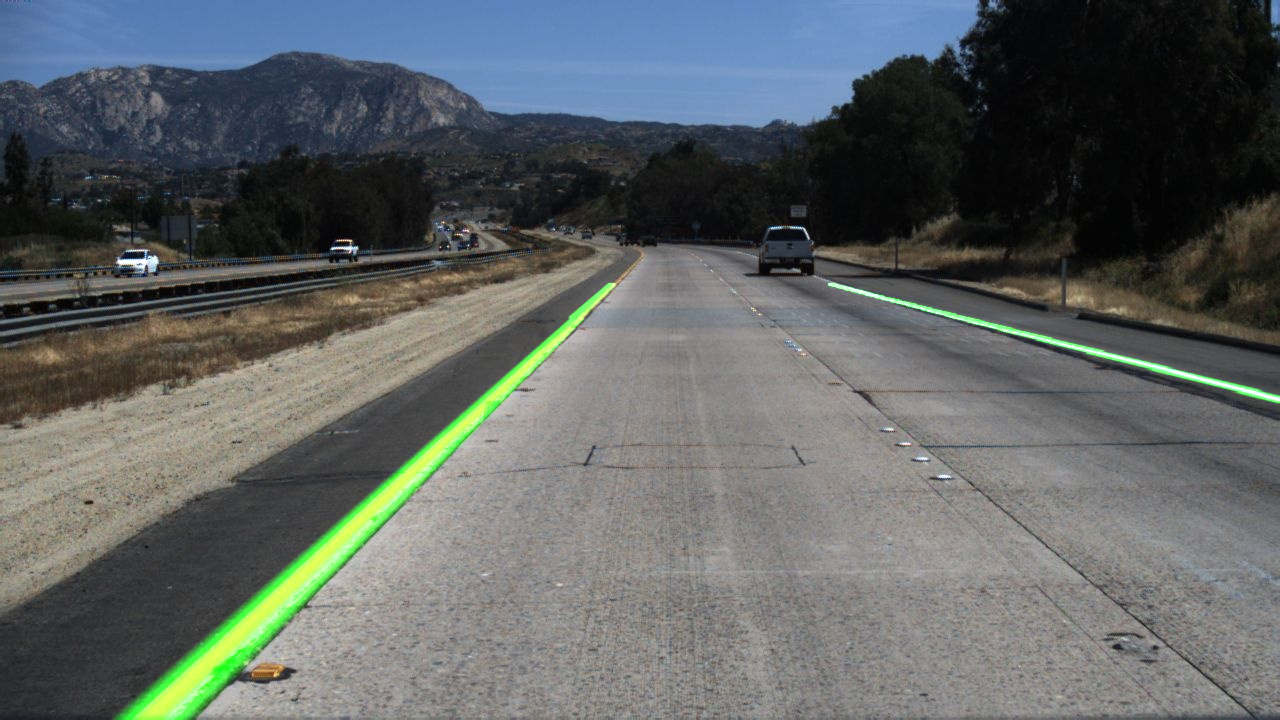
\includegraphics[width=0.48\textwidth]{img1.png}}
\hspace{0.03\textwidth}
\subfloat[]{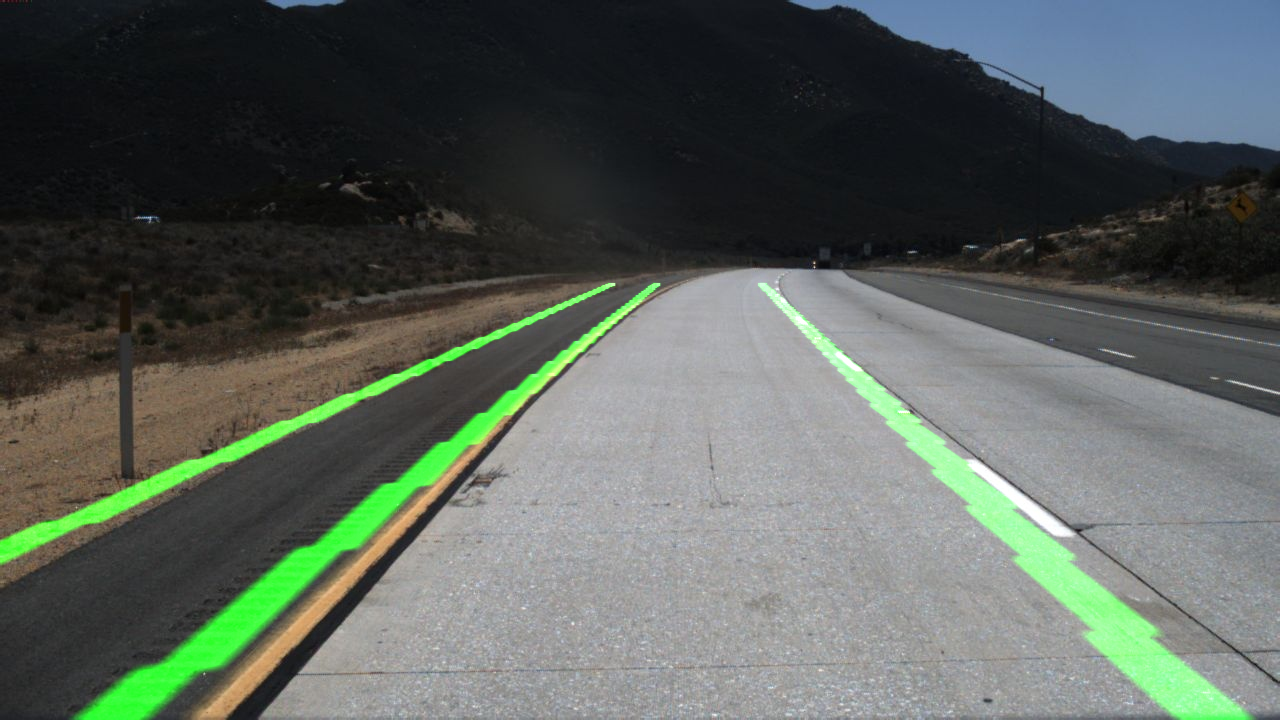
\includegraphics[width=0.48\textwidth]{img25.png}} \\

\subfloat[]{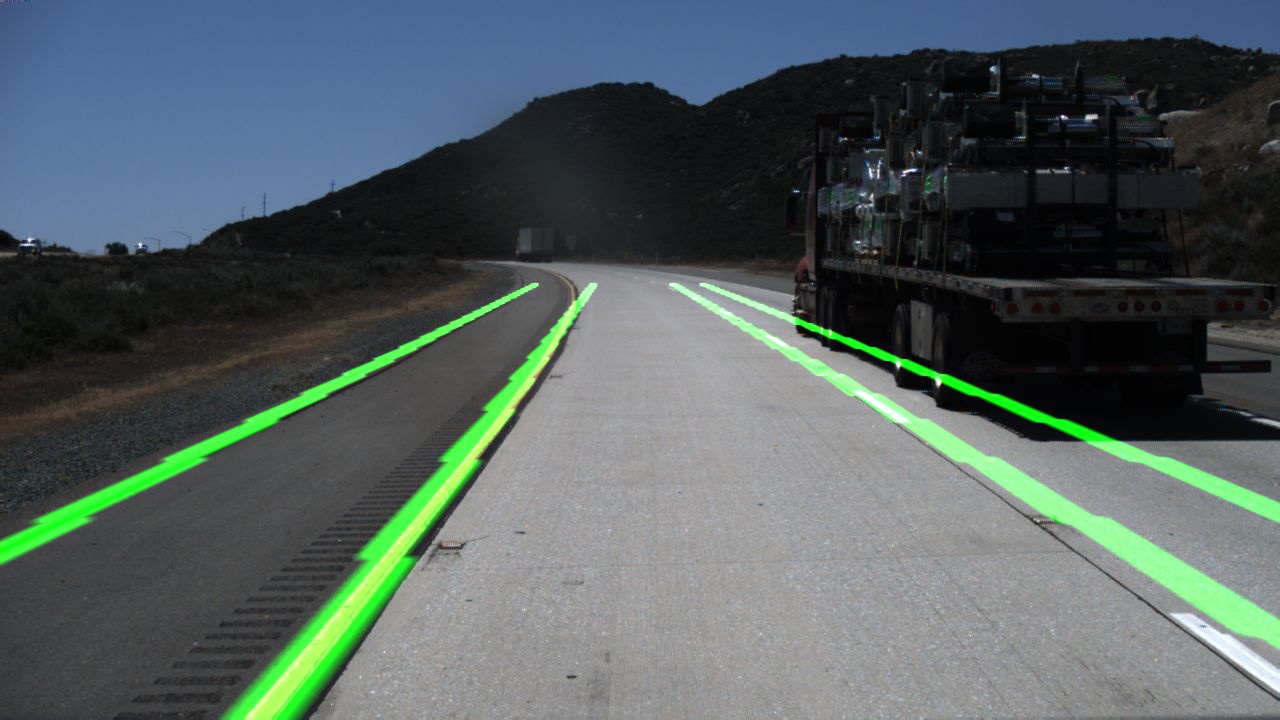
\includegraphics[width=0.48\textwidth]{img31.png}}
\hspace{0.03\textwidth}
\subfloat[]{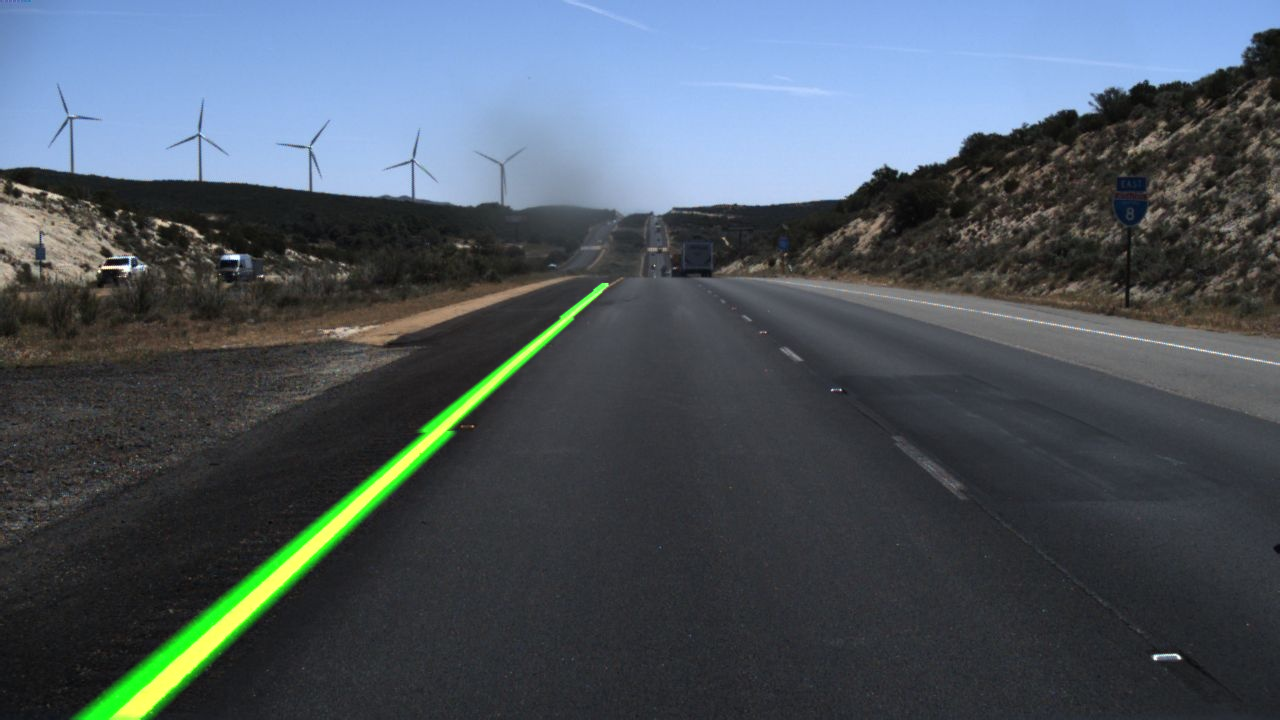
\includegraphics[width=0.48\textwidth]{img39.png}} \\

\subfloat[]{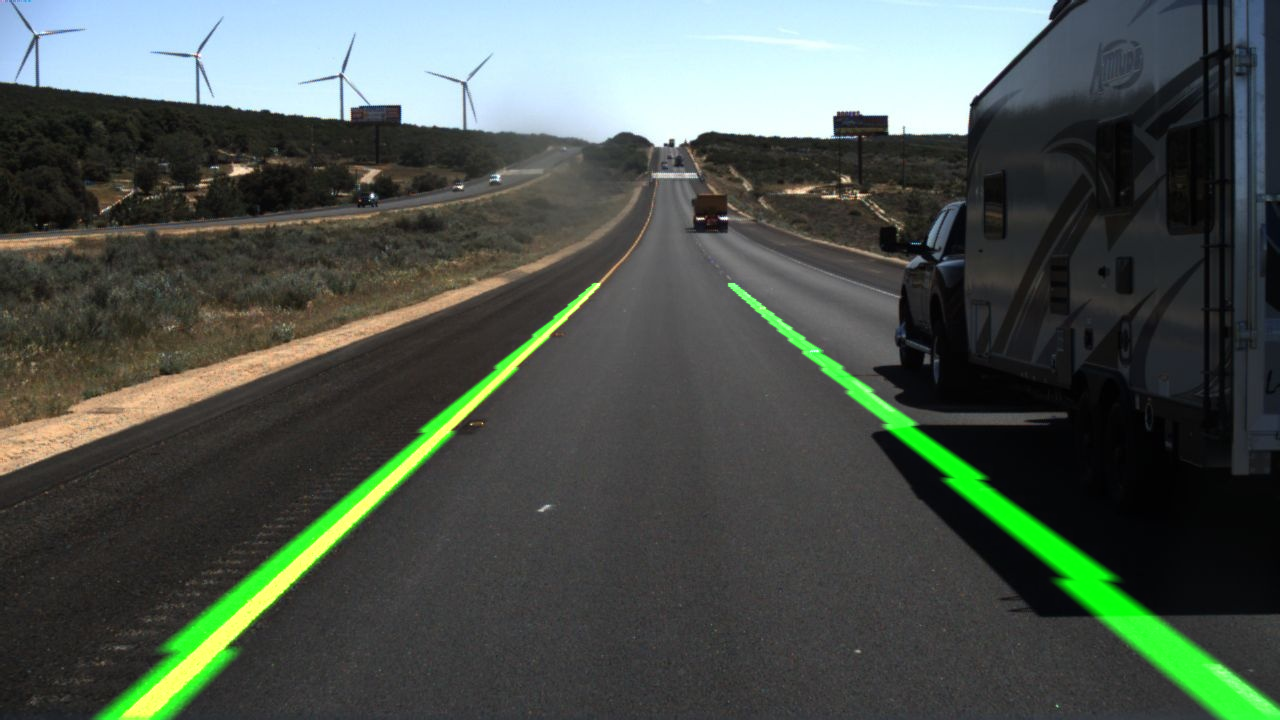
\includegraphics[width=0.48\textwidth]{img40.png}}
\hspace{0.03\textwidth}
\subfloat[]{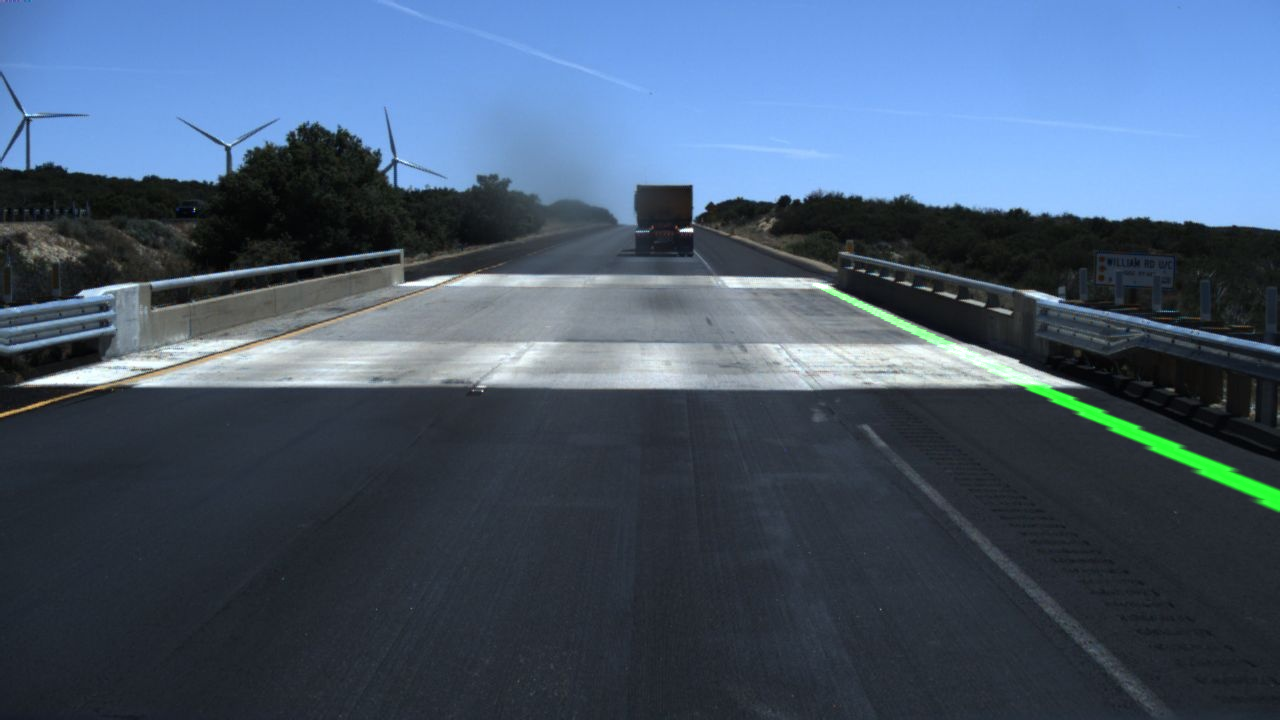
\includegraphics[width=0.48\textwidth]{img41.png}}

\caption{Примеры неверной работы алгоритма детектирования маркеров дорожной разметки на последовательности TuSimple. (a), (d), (f) -- некачественная разметка дорожного полотна. (e) -- полоса заслонена. (b), (c) -- ложные срабатывания.}
\label{fig:lane_det_fails}
\end{figure}

\newpage
\section{Заключение}

В рамках данной работы были достигнуты следующие результаты.

\begin{itemize}
\item На основе подхода Stixel World и классического стереозрения разработан и релизован на языке C++ прототип алгоритма решения задачи поиска препятствий движению автомобиля на изображении, полученном с помощью стереокамеры, закреплённой на лобовом стекле автомобиля с помощью карты диспаритета. Реализована модификация этого алгоритма для работы с неплотной картой диспаритета.

\item На основе методов классической обработки изображений разработан и реализован на языке Python прототип алгоритма поиска маркеров дорожной разметки на изображении, полученном с камеры, закреплённой на лобовом стекле автомобиля.

\item Выполнена апробация разработанных алгоритмов на наборах данных KITTI и TuSimple, а также на наборе данных Петергоф.

\end{itemize}

В качестве дальнейшего продолжения работы планируется предпринять следующие шаги.

\begin{itemize}
\item Разметить тестовый набор и проверить предположение об увеличении качества детектирования маркеров дорожной разметки при интеграции с алгоритмом детектирования препятствий.
\item Улучшить алгоритм детектирования маркеров дорожной разметки для случая нечётких маркеров.
\item Добавить синхронизацию предсказаний алгоритмов для последовательных кадров видеопоследовательности.
\end{itemize}

\newpage

\bibliographystyle{ugost2008ls}
\bibliography{diploma.bib}
\end{document}


